%%%%%%%%%%%%%%%%%%%%%%%%%%%%%%%%%%%%%%%%%%%%%%%%%%%%%%%%%%%%%%%%%%%%%%%%%%%%%%
%  Revisiting ViT-B Training and Post-Processing for Vehicle Re-Identification
%  Submission to: The Visual Computer (Springer)
%
%  FORMATTING NOTE
%  ---------------
%  The Visual Computer states in its Instructions for Authors that there is
%  currently no official journal template and that authors should follow the
%  generic Instructions for Authors; accepted papers are typeset by the
%  publisher.  This file therefore implements those instructions directly:
%    * single column, A4, 10 pt Times (via mathptmx / newtxtext)
%    * decimal headings, at most three levels
%    * numbered citations in square brackets, Springer reference style
%    * abstract 150-250 words, 4-6 keywords
%    * tables numbered in Arabic numerals with captions ABOVE the table
%    * figure captions beginning "Fig. N" in bold, no terminal punctuation
%    * Statements and Declarations section
%    * author biographies (50-100 words each)
%
%  To switch to Springer Nature's generic class instead, download sn-jnl.cls
%  from Springer and replace the \documentclass line with
%      \documentclass[sn-mathphys-num,iicol]{sn-jnl}
%  keeping the body text below unchanged.
%
%  Compile:  pdflatex manuscript && pdflatex manuscript
%  (Bibliography is embedded as thebibliography so no BibTeX run is needed.
%   A references.bib file is also provided if you prefer BibTeX; see the note
%   just above the bibliography at the end of this file.)
%%%%%%%%%%%%%%%%%%%%%%%%%%%%%%%%%%%%%%%%%%%%%%%%%%%%%%%%%%%%%%%%%%%%%%%%%%%%%%

\documentclass[10pt,a4paper]{article}

% ---- Page layout -------------------------------------------------------------
\usepackage[a4paper,margin=1in]{geometry}
\usepackage[T1]{fontenc}
\usepackage[utf8]{inputenc}
\usepackage{mathptmx}                 % Times text and math
\usepackage[scaled=0.90]{helvet}      % Helvetica for figure/sans elements

% ---- Maths, tables, graphics -------------------------------------------------
\usepackage{amsmath,amssymb,amsfonts}
\usepackage{booktabs}
\usepackage{multirow}
\usepackage{array}
\usepackage{graphicx}
\usepackage{xcolor}
\usepackage{pifont}
\graphicspath{{figs/}}
\usepackage{wrapfig}
% ---- Typography, captions, links --------------------------------------------
\usepackage{microtype}
\usepackage[font=small,labelfont=bf,labelsep=space]{caption}
\usepackage{url}
\usepackage[hidelinks,breaklinks=true]{hyperref}
\usepackage{fancyhdr}
\usepackage{titlesec}

\setlength{\parskip}{0pt}
\setlength{\tabcolsep}{4pt}
\renewcommand{\arraystretch}{1.08}

% Figure captions must read "Fig. 1 ..." with no terminal punctuation
\renewcommand{\figurename}{Fig.}
\captionsetup[figure]{name=Fig.}
\captionsetup[table]{name=Table}

% Decimal headings, three levels maximum
\titleformat{\section}{\normalfont\large\bfseries}{\thesection}{0.6em}{}
\titleformat{\subsection}{\normalfont\normalsize\bfseries}{\thesubsection}{0.6em}{}
\titleformat{\subsubsection}{\normalfont\normalsize\itshape}{\thesubsubsection}{0.6em}{}
\setcounter{secnumdepth}{3}

\newcommand{\cmark}{\ding{51}}
\newcommand{\xmark}{\ding{55}}
\newcolumntype{L}[1]{>{\raggedright\arraybackslash}p{#1}}
\newcolumntype{C}[1]{>{\centering\arraybackslash}p{#1}}

\pagestyle{fancy}
\fancyhf{}
\renewcommand{\headrulewidth}{0pt}
\fancyfoot[C]{\thepage}

% =============================================================================
\begin{document}
% =============================================================================

% ---- Title page -------------------------------------------------------------
\begin{center}
  {\LARGE\bfseries Revisiting ViT-B Training and Post-Processing for Vehicle
  Re-Identification: A Reproducible Baseline and Training-Free Fusion on
  VeRi-776\par}

  \vspace{1.4em}

  {\normalsize
   Seif T. Heakal$^{1,\ast}$ \quad
   Mohamed A. Ali$^{1}$ \quad
   Ali A. Ali$^{1}$ \\[4pt]
   Abdelrahman Hamdi$^{1}$ \quad
   Ahmed H. Abdel-Gawad$^{1}$\par}

  \vspace{0.9em}

  {\small $^{1}$\,Department of Computer Engineering, Faculty of Engineering,
   Cairo University, Giza 12613, Egypt\par}

  \vspace{0.5em}

  {\small $^{\ast}$\,Corresponding author:
   \texttt{seif.mohamed05@eng-st.cu.edu.eg}\par}

  \vspace{0.4em}

  {\footnotesize
    \texttt{seif.mohamed05@eng-st.cu.edu.eg};\;
    \texttt{mohamed.awaad02@eng-st.cu.edu.eg};\\
   \texttt{ali.abdelraouf03@eng-st.cu.edu.eg};\;
   \texttt{abdelrahman.ibrahim03@eng-st.cu.edu.eg};\;
   \texttt{ahamdy@eng.cu.edu.eg}\par}

  \vspace{0.4em}

  {\footnotesize ORCID: [to be supplied by each author at submission]\par}
\end{center}

\vspace{1.0em}

% ---- Abstract (150-250 words per the Instructions for Authors) ---------------
% ===== UNIT 01: Abstract =====
% Status: AI-DRAFT  (change to REWRITTEN / REVIEWED when done; see CHECKLIST.md)
% Rules: keep every \cite, \ref, \label, number and table value unless you checked it against the logs.
\noindent\textbf{Abstract}\\[4pt]
{\small
Transformer backbones dominate vehicle re-identification (Re-ID), yet their
training recipes and evaluation-time post-processing are rarely reported under
matched conditions, which makes it difficult to attribute reported progress to
any specific cause. This paper revisits the ViT-Base/16 pipeline on VeRi-776
and separates recipe effects from post-processing effects. A fully specified
recipe---CLIP-pretrained initialisation, AdamW with layer-wise learning-rate
decay, a tuned metric objective, and a three-step post-processing chain of
average query expansion, $k$-reciprocal re-ranking and flip test-time
augmentation---reaches 89.97\% mAP and 97.79\% Rank-1. A matched-condition
experiment shows that this figure is produced by post-processing rather than by
the recipe: at the raw-embedding level the recipe merely matches TransReID
(82.22 versus 82.30\% mAP), and applying the identical post-processing to the
official TransReID and CLIP-ReID checkpoints lifts them to 91.12 and 91.80\%
mAP, both above ours. We therefore present this stream as a reproducible
baseline, not a superior recipe. A training-free score-level fusion of this
stream with CLIP-SENet reaches 93.32\% mAP and 98.45\% Rank-1, exceeding the
best previously published mAP by 0.42\,pp, with a paired bootstrap confirming a
statistically significant gain over the stronger single stream. A zero-shot
transfer study across all three VeRi-Wild protocols shows the ViT-B embedding
transfers competitively while the fusion and re-ranking gains do not,
indicating that they are domain-specific. Checkpoints, notebooks and per-query
dumps are released for deterministic re-computation.
\par}


\vspace{0.8em}
\noindent{\small\textbf{Keywords}\; Vehicle re-identification $\cdot$
Vision Transformer $\cdot$ Score-level fusion $\cdot$ $k$-reciprocal
re-ranking $\cdot$ VeRi-776 $\cdot$ Cross-dataset generalisation}

\vspace{1.2em}

% =============================================================================
\section{Introduction}
\label{sec:intro}
% =============================================================================

% ===== UNIT 02: Motivation (1.1) =====
% Status: REWRITTEN  (change to REWRITTEN / REVIEWED when done; see CHECKLIST.md)
% Rules: style rewrite only. Keep every \cite, \ref, \label, number, equation and table value as is. Change the wording, not the content.
\subsection{Motivation}
Vehicle re-identification is heavily used in intelligent
transportation systems (ITS), supporting applications including urban traffic
surveillance, law enforcement and smart city infrastructure~\cite{liu2016veri,liu2018provid}.
The task requires matching the
same physical vehicle across multiple spatially distributed cameras whose
fields of view do not overlap. The same vehicle can look very different: it may be observed from different angles, under
different illumination conditions, at varying resolutions, and after arbitrary
time intervals~\cite{liu2016veri}.

The VeRi-776 dataset~\cite{liu2016veri,liu2018provid}, introduced by Liu
\emph{et al.} in 2016 and expanded by the PROVID framework published
in \emph{IEEE Transactions on Multimedia} in 2018, has become the
benchmark for vehicle ReID evaluation. It contains over 50\,000 images of 776
vehicles captured by 20 cameras covering a $1.0\,\text{km}^{2}$ urban area over
24 hours, with each vehicle appearing in 2 to 18 cameras under varied
viewpoints, illuminations, and occlusions~\cite{liu2016veri,liu2018provid}. The
standard evaluation protocol employs 37\,781 training images of 576
identities, 11\,579 gallery images, and 1\,678 query images across 200 test
identities~\cite{liu2018provid}. Performance is measured by mean Average
Precision (mAP) and Rank-1 Cumulative Matching Characteristic (CMC).


% ===== UNIT 03: The ViT-B training recipe gap (1.2) =====
% Status: REWRITTEN  (change to REWRITTEN / REVIEWED when done; see CHECKLIST.md)
% Rules: style rewrite only. Keep every \cite, \ref, \label, number, equation and table value as is. Change the wording, not the content.
\subsection{The ViT-B training recipe gap}
The introduction of TransReID~\cite{he2021transreid} changed how people approached
vehicle ReID by applying a pure Vision Transformer
(ViT)~\cite{dosovitskiy2021vit} backbone to the task. TransReID augments the
standard ViT-B/16 architecture with two extra modules: the Side
Information Embedding (SIE), which encodes camera index and viewpoint as
learnable token offsets to reduce domain bias, and the Jigsaw Patch Module
(JPM), which shuffles patch tokens in a parallel branch to force the model to learn local
features~\cite{he2021transreid}. With a DeiT-B/16 backbone and SGD
(momentum 0.9, LR 0.008, cosine decay), TransReID reports 82.3\% mAP and 97.1\%
Rank-1 on VeRi-776~\cite{he2021transreid}.

Despite broad adoption of this architecture as a baseline, subsequent work has
primarily focused on augmenting it with new architectural
components: semantic alignment via language
models~\cite{li2023clipreid,lu2025clipsenet}, graph-based spatial
reasoning~\cite{shen2022hpgn}, or multi-branch CNN
structures~\cite{luo2023mbr4b}, instead of looking again at what a
properly tuned ViT-B training-and-post-processing pipeline leaves on the table.
No pure ViT-B method has been reported above 90\% mAP on VeRi-776. We push a
pure ViT-B/16 pipeline to 89.97\% mAP, approaching that mark, and, via
training-free fusion with a complementary CNN-semantic stream, reach 93.3\%.



% ===== UNIT 04: Contributions + paper organisation (1.3-1.4) =====
% Status: REWRITTEN  (change to REWRITTEN / REVIEWED when done; see CHECKLIST.md)
% Rules: style rewrite only. Keep every \cite, \ref, \label, number, equation and table value as is. Change the wording, not the content.
\subsection{Contributions}
The contributions of this work are as follows:
\begin{itemize}
  \item \textbf{C1: Reproducible ViT-B/16 pipeline and a
    recipe-versus-post-processing analysis.} We release a specific
    ViT-B/16 retrieval pipeline (CLIP initialisation, a tuned metric objective,
    an optimised augmentation pipeline, AQE $+$ $k$-reciprocal
    re-ranking~\cite{zhong2017rerank}, flip TTA) reaching \textbf{89.97\% mAP /
    97.79\% Rank-1} on VeRi-776. We test what drives this
    number: applying our identical post-processing to the official TransReID
    and CLIP-ReID checkpoints lifts them to \textbf{91.12\%} and
    \textbf{91.80\% mAP}, both slightly above ours, while all three
    are within 0.9\,pp without post-processing
    (82.11\,/\,82.99\,/\,82.22\%, Table~\ref{tab:matched}). Our recipe thus
    gives no advantage over these baselines at matched conditions: the ViT-B
    retrieval gains are because of post-processing, and we position
    Stream~1 as a reproducible baseline, not a superior recipe. Among
    single models reported with post-processing, MBR4B-LAI
    (92.1\% mAP~\cite{luo2023mbr4b}) is also higher.
  \item \textbf{C2: Marginal new best mAP via training-free fusion.}
    Score-level fusion with CLIP-SENet~\cite{lu2025clipsenet} achieves
    \textbf{93.32\% mAP / 98.45\% Rank-1}, $+0.42$\,pp mAP above the best
    previously published result (92.9\%~\cite{lu2025clipsenet}) and
    $+1.88$\,pp above our own reproduction of that stream (91.44\%). Rank-1
    (98.45\%) is competitive with but does not exceed CLIP-SENet standalone
    Rank-1 (98.7\%). Because the $+0.42$\,pp margin is small and our fusion reuses that model's
    released checkpoint, we present it as a demonstration of feature
    complementarity, not a decisive state of the art. A paired bootstrap test
    shows that the gain over the best single stream is significant
    (Section~\ref{sec:holdout}).
  \item \textbf{C3: Same-setup ablation path.} An in depth
    ablation traces the complete performance trajectory from the 82.3\%
    TransReID baseline to 93.3\% mAP under a single consistent post-processing
    protocol, separating post-processing contributions from recipe
    contributions instead of conflating them.
  \item \textbf{C4: Reproducible public release with validation and cost
    analysis.} All checkpoints (SHA-256 pinned), evaluation notebooks,
    configuration files, per-query evaluation dumps, and the post-processing
    pipeline are publicly released. Every reported number is the deterministic
    re-evaluation of a frozen, hash-pinned checkpoint and is thus
    exactly re-computable from the release. From-scratch retraining is
    reproducible within a $\pm0.55$\,pp seed band
    (Section~\ref{sec:seed_variance}). Headline numbers use hyperparameters
    selected on the standard evaluation split (disclosed, not implicit), with
    held-out validation bounding the resulting optimism to $\leq$0.2\,pp mAP
    (Section~\ref{sec:holdout}), and the latency and memory of every pipeline
    stage (extraction, TTA, AQE, re-ranking, fusion) are measured for
    deployment planning (Section~\ref{sec:cost}).
  \item \textbf{C5: Cross-dataset transfer study.} A zero-shot
    VeRi-776$\rightarrow$VeRi-Wild evaluation across all three official test
    protocols (with paired-bootstrap CIs and released per-query dumps) shows
    the ViT-B stream transfers competitively with published cross-domain
    methods that use over twenty times more source identities or adapt using
    unlabelled target data, while the two-stream fusion does not
    transfer at any scale: evidence, supported by a CityFlowV2 MTMC port,
    that its VeRi-776 advantage is domain-specific
    (Section~\ref{sec:veriwild}).
\end{itemize}

\subsection{Paper organisation}
Section~\ref{sec:related} reviews related work across CNN-era methods,
transformer-based methods, and post-processing techniques.
Section~\ref{sec:method} describes the full methodology including both streams
and the fusion strategy. Section~\ref{sec:setup} details the experimental
setup. Section~\ref{sec:results} presents quantitative results and ablations.
Section~\ref{sec:discussion} discusses findings and limitations.
Section~\ref{sec:conclusion} concludes.


\subsection{Paper organisation}
Section~\ref{sec:related} reviews related work across CNN-era methods,
transformer-based methods, and post-processing techniques.
Section~\ref{sec:method} describes the full methodology including both streams
and the fusion strategy. Section~\ref{sec:setup} details the experimental
setup. Section~\ref{sec:results} presents quantitative results and ablations.
Section~\ref{sec:discussion} discusses findings and limitations.
Section~\ref{sec:conclusion} concludes.

% =============================================================================
\section{Related work}
\label{sec:related}
% =============================================================================

% ===== UNIT 05: CNN-era vehicle re-ID (2.1) =====
% Status: AI-DRAFT  (change to REWRITTEN / REVIEWED when done; see CHECKLIST.md)
% Rules: keep every \cite, \ref, \label, number and table value unless you checked it against the logs.
\subsection{CNN-era vehicle re-identification}
The VeRi-776 benchmark was introduced by Liu et al.~\cite{liu2016veri} and
extended with the PROVID framework~\cite{liu2018provid}, which combined visual
appearance, licence plate recognition, camera topology, and spatiotemporal
cues, achieving 53.42\% mAP and 81.56\% Rank-1.\footnote{The PROVID
(53.42/81.56) and VAMI (50.13/77.03) figures are the values reported in the
respective papers and reproduced throughout the survey
literature~\cite{ye2022survey,li2024vehiclereidsurvey}.} A broad survey of deep
learning approaches to person and vehicle ReID is provided by Ye et
al.~\cite{ye2022survey}, while Li et al.~\cite{li2024vehiclereidsurvey} survey
vehicle-specific advances including part-level modelling, multi-source
training, and cross-domain adaptation.

VAMI~\cite{zhou2018vami} (CVPR 2018) synthesised target viewpoints via
adversarial training, reaching 50.13\% mAP and 77.03\% Rank-1.
PVEN~\cite{meng2020pven} (CVPR 2020) introduced parsing-based view-aware
embeddings via semantic segmentation for part-level feature extraction,
achieving 79.5\% mAP and 95.6\% Rank-1. CAL~\cite{rao2021cal} (ICCV 2021)
proposed counterfactual attention learning to suppress spurious background
cues, reaching 74.3\% mAP and 95.4\% Rank-1.
VehicleNet~\cite{zheng2020vehiclenet} (IEEE TMM 2020) demonstrated
multi-source data aggregation across VeRi-776, VehicleID, and synthetic data,
achieving 83.41\% mAP and 96.78\% Rank-1. HPGN~\cite{shen2022hpgn} (IEEE T-ITS
2022) modelled spatial significance across image scales via a pyramid graph
network, achieving 80.18\% mAP and 96.72\% Rank-1. A Strong
Baseline~\cite{cybercore2021strong} (CVPR-W AICity 2021) combined
ResNet101-IBN-a with multi-head attention for multi-domain training, reaching
87.1\% mAP and establishing a competitive ResNet-family ceiling prior to
transformer approaches. Khorramshahi et
al.~\cite{khorramshahi2023selfsupervision} later revisited scalable vehicle
ReID through self-supervised pretraining across ResNet, ViT, Swin, and ConvNeXt
backbones in the AI City setting.


% ===== UNIT 06: Transformer-based vehicle re-ID (2.2) =====
% Status: REWRITTEN  (change to REWRITTEN / REVIEWED when done; see CHECKLIST.md)
% Rules: style rewrite only. Keep every \cite, \ref, \label, number, equation and table value as is. Change the wording, not the content.
\subsection{Transformer-based vehicle re-identification}
TransReID~\cite{he2021transreid} (ICCV 2021) was the first pure Vision Transformer framework for object re-identification. It introduced the SIE and JPM modules. It gets 82.3\% mAP and 97.1\% Rank-1 on VeRi-776 with SGD. We switch the initialisation from ImageNet-21k to CLIP~\cite{radford2021clip} and the optimiser from SGD to AdamW~\cite{loshchilov2019adamw}. This gives a large gain in our own development, with no change to the architecture. Section~\ref{sec:matched} shows that it is not a net gain over the tuned published baseline.

CLIP-ReID~\cite{li2023clipreid} (AAAI 2023) uses a two-stage prompt-tuning procedure. It uses the vision-language knowledge in CLIP and needs no text annotations. It gets 84.5\% mAP and 97.3\% Rank-1 on VeRi-776~\cite{opencodepapers2024veri}. CLIP-ReID uses the same ViT-B/16 CLIP backbone family as our work. Our full pipeline reaches 89.97\% mAP, but this is not a matched comparison. CLIP-ReID's 84.5\% is reported without post-processing. At the raw-embedding level it is higher than our recipe (84.5\% vs.\ 82.2\%). The difference in the pipeline number comes from post-processing, which means AQE $+$ $k$-reciprocal re-ranking $+$ TTA. We apply it and the CLIP-ReID figure does not include it (Section~\ref{sec:discussion}). Recent transformer papers go beyond single-domain VeRi retrieval. MSFFT~\cite{holla2024msfft} fuses multi-scale transformer features for cross-platform vehicle ReID. MiKeCoCo~\cite{kuang2025mikecoco} uses CLIP-guided prompt knowledge to make vehicle ReID generalise better.

RPTM~\cite{ghosh2023rptm} (WACV 2023) uses relation-preserving triplet mining. It makes triplet loss training more stable across hard and semi-hard negatives. It gets 88.0\% mAP and 97.3\% Rank-1. MBR4B-LAI~\cite{luo2023mbr4b} (ITSC 2023) combines four convolutional branches with location-aware identity embeddings and camera and pose metadata. It reaches 92.09\% mAP and 98.03\% Rank-1 after re-ranking. This is a strong CNN ensemble, and our fusion method beats it. FastReID~\cite{wang2020fastreid} is a unified, production-quality baseline toolbox. People use it widely for ablations and comparisons across vehicle and person ReID benchmarks.

CLIP-SENet~\cite{lu2025clipsenet} (IEEE T-ITS 2026) is a single-stream approach. It combines ResNet101-IBN-a local appearance features with 512-dimensional semantic embeddings. The embeddings come from a TinyCLIP Semantic Extraction Module (SEM) and an Adaptive Fine-Grained Enhancement Module (AFEM). It gets 92.9\% mAP and 98.7\% Rank-1 on VeRi-776. This is the closest prior result to ours. We take the pre-trained CLIP-SENet v6 checkpoint as a frozen second stream. We fuse the two streams at score level with no training. This adds $+0.42$\,pp mAP above the CLIP-SENet standalone result.


% ===== UNIT 07: Cross-domain transfer and dataset bias (2.3) =====
% Status: REWRITTEN  (change to REWRITTEN / REVIEWED when done; see CHECKLIST.md)
% Rules: style rewrite only. Keep every \cite, \ref, \label, number, equation and table value as is. Change the wording, not the content.
\subsection{Cross-domain transfer and dataset bias}
Cross-dataset transfer is a known weak point of ReID systems. Unsupervised domain adaptation (UDA) methods such as SPGAN~\cite{deng2018spgan}, ECN~\cite{zhong2019ecn} and UDAP~\cite{song2020udap} train on a labelled source and adapt using unlabelled target data. They are trained on the large VehicleID source and tested on VeRi-Wild. On the 3{,}000-identity protocol they reach 24.1--34.7\% mAP. The strongest reported direct transfer (no target data at all) reaches 37.7\%. Full viewpoint-aware adaptation reaches 39.7\%~\cite{zheng2020vapc}. Recent work finds that much of the gap between in-domain and cross-domain performance comes from train/test similarity bias inside the ReID benchmarks. Models trained on VeRi-Wild lose ${\approx}15$\,pp mAP when tested on the visually similar VeRi-776. The mAP on vehicle types unseen during training drops from above 90\% to 65--70\%, even for state-of-the-art models~\cite{benmabrouk2026genlimits}. This is the context for the cross-dataset evaluation in Section~\ref{sec:veriwild}. Large drops under zero-shot transfer are normal in this field. They do not come from one particular pipeline.


% ===== UNIT 08: Re-ranking and post-processing (2.4) =====
% Status: AI-DRAFT  (change to REWRITTEN / REVIEWED when done; see CHECKLIST.md)
% Rules: style rewrite only. Keep every \cite, \ref, \label, number, equation and table value as is. Change the wording, not the content.
\subsection{Re-ranking and post-processing}
The $k$-reciprocal encoding method by Zhong et al.~\cite{zhong2017rerank} (CVPR
2017) leverages the observation that if a gallery image lies in the
$k$-reciprocal nearest neighbours of a probe, it is more likely to be a true
match. A Jaccard-distance-based score is blended with the original cosine
distance, improving retrieval precision without requiring labelled data. Zhang
et al.~\cite{zhang2022vehiclererank} extended this idea specifically for
vehicle ReID by incorporating orientation-guided query expansion, showing that
viewpoint-consistent neighbour selection further improves re-ranking for highly
viewpoint-sensitive queries. Moral et al.~\cite{moral2023syntheticrerank} also
studied vehicle-specific post-processing, including gallery video-clip
information in the re-ranking step on CityFlow-ReID and VeRi-776.

Average Query Expansion (AQE)~\cite{arandjelovic2012aqe} replaces each query
feature with the mean of its top-$k$ retrieved gallery features, smoothing the
query manifold and consistently improving mAP at negligible computational cost.
Database-side Augmentation (DBA) applies the same expansion to gallery features
and can be combined with AQE; we evaluate AQE alone as it provides the best
mAP--Rank-1 trade-off at $k{=}3$ for our ViT-B stream.

Supervised Contrastive Learning (SupCon)~\cite{khosla2020supcon} extends
contrastive losses to the supervised setting by treating all same-class samples
as positives within each mini-batch, producing more uniformly distributed and
discriminative embedding spaces than triplet loss alone~\cite{ye2022survey}. We
evaluate SupCon as an alternative metric objective for Stream~1 (variant
A5$\beta$); the deployed checkpoint (A5$\alpha$) retains a triplet $+$ centre
objective, and the two are shown to be statistically equivalent
(Section~\ref{sec:seed_variance}).


% ===== UNIT 09: Positioning (2.5) =====
% Status: REWRITTEN  (change to REWRITTEN / REVIEWED when done; see CHECKLIST.md)
% Rules: style rewrite only. Keep every \cite, \ref, \label, number, equation and table value as is. Change the wording, not the content.
\subsection{Positioning}
To the best of our knowledge, no prior work reports above 90\% mAP on VeRi-776 with a pure ViT-B backbone. The best prior pure-ViT result is 84.5\% mAP~\cite{li2023clipreid,opencodepapers2024veri}, reported without post-processing. Our ViT-B pipeline reaches 89.97\% mAP, but this is not a like-for-like comparison. The 84.5\% is a raw-embedding number. The 89.97\% includes AQE $+$ $k$-reciprocal re-ranking $+$ TTA. Without post-processing, our embedding (82.2\% mAP) does not beat CLIP-ReID. The matched comparison shows that the gain comes from post-processing. We apply our identical post-processing to the official TransReID and CLIP-ReID checkpoints. They reach \textbf{91.12\%} and \textbf{91.80\% mAP}, both above our 89.97\%. So our recipe has no advantage over either baseline (Section~\ref{sec:matched}). For the fusion result, no prior two-stream method exceeds 93.3\% mAP on VeRi-776. The best prior single-stream result is 92.9\% mAP~\cite{lu2025clipsenet}. Our fusion beats it by a narrow $+0.42$\,pp.


% =============================================================================
\section{Methodology}
\label{sec:method}
% =============================================================================

% ===== UNIT 10: Overview figure + problem formulation (3.1) =====
% Status: AI-DRAFT  (change to REWRITTEN / REVIEWED when done; see CHECKLIST.md)
% Rules: style rewrite only. Keep every \cite, \ref, \label, number, equation and table value as is. Change the wording, not the content.
Figure~\ref{fig:arch} gives the overall architecture of the two-stream
pipeline, from image input through per-stream feature extraction and
post-processing to score-level fusion, together with the two operating points
reported in this paper.

\begin{figure*}[!t]
  \centering
  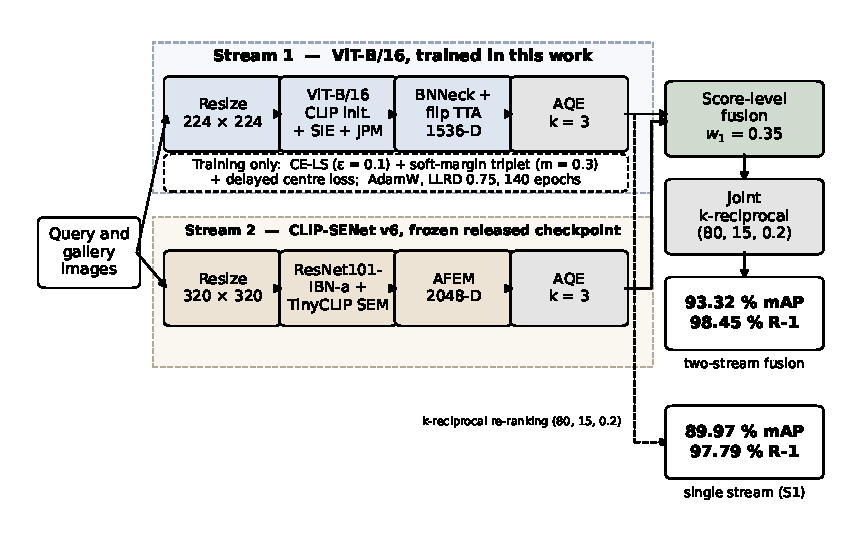
\includegraphics[width=\textwidth]{Fig1}
  \caption{Overview of the two-stream pipeline. Stream~1 (top) is the ViT-B/16
  backbone trained in this work; Stream~2 (bottom) is the frozen, publicly
  released CLIP-SENet v6 checkpoint. Average query expansion is applied to each
  stream, the resulting cosine-similarity matrices are combined by a weighted
  sum, and a single joint $k$-reciprocal re-ranking pass is applied to the
  fused matrix. The dashed path shows the single-stream operating point, in
  which Stream~1 is re-ranked on its own}
  \label{fig:arch}
\end{figure*}

\subsection{Problem formulation}
Given a query image $q$ and a gallery set
$\mathcal{G} = \{g_1, g_2, \ldots, g_N\}$, the task is to retrieve all gallery
images depicting the same vehicle identity as the query and rank them above
non-matching images. Performance is measured by mAP and Rank-1 CMC. The
standard VeRi-776 evaluation protocol~\cite{liu2018provid} employs 1\,678 query
images and 11\,579 gallery images across 200 test identities; training uses
37\,781 images of 576 identities. All reported results strictly follow this
protocol.


\subsection{Stream~1: improved ViT-B training recipe}

% ===== UNIT 11: Stream 1: backbone architecture (3.2.1) =====
% Status: REWRITTEN  (change to REWRITTEN / REVIEWED when done; see CHECKLIST.md)
% Rules: style rewrite only. Keep every \cite, \ref, \label, number, equation and table value as is. Change the wording, not the content.
\subsubsection{Backbone architecture}
The backbone follows the TransReID architecture~\cite{he2021transreid}. It is a ViT-Base/16 with the SIE module and the JPM added. The SIE module encodes the 20 camera indices of VeRi-776 as learnable offsets, which are added to the patch token sequence. The JPM is a parallel branch. It randomly shuffles groups of patch tokens and uses a separate classification head. A BNNeck is applied on the 768-dimensional global CLS token, before the classification head~\cite{he2021transreid}.

The main difference from the original TransReID recipe is the backbone initialisation. We use \texttt{vit\_base\_\allowbreak patch16\_\allowbreak clip\_\allowbreak
224.openai} (OpenAI CLIP pretrained ViT-B/16 via
\texttt{timm}~\cite{radford2021clip}). It replaces the ImageNet-21k-only weights. CLIP pretraining gives richer visual and semantic features. They transfer better to fine-grained vehicle appearance.


% ===== UNIT 12: Stream 1: loss function + equations (3.2.2) =====
% Status: REWRITTEN  (change to REWRITTEN / REVIEWED when done; see CHECKLIST.md)
% Rules: style rewrite only. Keep every \cite, \ref, \label, number, equation and table value as is. Change the wording, not the content.
\subsubsection{Loss function}
Training uses a composite loss. The classification loss is cross-entropy
with label smoothing ($\varepsilon = 0.1$):
\begin{equation}
  \mathcal{L}_{\mathrm{CE\text{-}LS}} =
    -\sum_{c=1}^{C} y_c^{\mathrm{smooth}} \log \hat{p}_c, \;\;
    y_c^{\mathrm{smooth}} = (1{-}\varepsilon)y_c + \varepsilon/C
  \label{eq:cels}
\end{equation}
where $C = 576$ training identities. The recipe of the released headline checkpoint
(A5$\alpha$) adds two terms to this loss. One is a soft-margin triplet loss
(margin $m{=}0.3$). The other is a delayed centre loss ($\lambda{=}5\times10^{-4}$),
enabled after epoch~30. We also use layer-wise learning-rate decay of 0.75:
\begin{equation}
  \mathcal{L}_{\mathrm{A5\alpha}} =
    \mathcal{L}_{\mathrm{CE\text{-}LS}}
    + \mathcal{L}_{\mathrm{tri}}(m{=}0.3)
    + \lambda\,\mathcal{L}_{\mathrm{centre}}
  \label{eq:a5alpha}
\end{equation}
We also evaluate an alternative, a supervised-contrastive variant (A5$\beta$).
It replaces the triplet and centre terms with Supervised Contrastive Loss
(SupCon)~\cite{khosla2020supcon} ($\tau = 0.07$, LLRD 0.65):
\begin{equation}
  \mathcal{L}_{\mathrm{SupCon}} =
    \sum_{i \in \mathcal{B}}
      \frac{-1}{|\mathcal{P}(i)|}
      \sum_{p \in \mathcal{P}(i)}
        \log
        \frac{\exp(\mathbf{z}_i \cdot \mathbf{z}_p / \tau)}
             {\sum_{a \in \mathcal{A}(i)} \exp(\mathbf{z}_i \cdot \mathbf{z}_a / \tau)}
  \label{eq:supcon}
\end{equation}
where $\mathcal{P}(i)$ is the set of positive pairs and $\mathcal{A}(i)$ is all
other mini-batch samples. This gives
$\mathcal{L}_{\mathrm{A5\beta}} = \mathcal{L}_{\mathrm{CE\text{-}LS}} +
\mathcal{L}_{\mathrm{SupCon}}$. A5$\alpha$ and A5$\beta$ are separate ablation rows.
In single from-scratch ablation runs, A5$\alpha$ gets 89.06\% mAP and A5$\beta$ gets 88.57\% mAP
under stream-1-only AQE$+$rerank evaluation (the released A5$\alpha$ checkpoint scores 89.63\% at this setting). The difference is 0.49\,pp, with A5$\alpha$ higher.
This is well inside the $\pm 0.55$\,pp three-seed standard deviation of
A5$\alpha$ (88.75 $\pm$ 0.55\,pp mAP, see Table~\ref{tab:ablation} and
Section~\ref{sec:seed_variance}). So the two recipes are statistically equivalent.
We keep A5$\alpha$ as the headline Stream~1 recipe, because the released checkpoint was trained with it.

CircleLoss made training unstable in our full-recipe runs. The training loss diverged,
so we leave it out of the final recipe. To find the cause, we ran a controlled 400-step
diagnostic with a minimal head (plain CLIP-initialised ViT-B $+$ BNNeck $+$ CE-LS $+$ metric loss,
$P{\times}K=12{\times}8$). We tested five conditions. These were CircleLoss at
$\gamma\in\{32,64\}$ under fp16 and fp32, an ImageNet-initialised control, and
a triplet$+$centre control. None of the CircleLoss conditions diverged
in this minimal setting. The fp16 and fp32 runs differed only in descent speed.
CLIP and ImageNet initialisation behaved similarly. So neither precision nor
initialisation is a simple explanation. The instability we saw is specific to the
full recipe (SIE/JPM heads, layer-wise learning-rate decay and the longer schedule).
It does not come from CircleLoss on CLIP features alone. We did not isolate the exact cause.
CircleLoss stays excluded because of what we observed in the full setting.
The probe script and loss curves are released with the code.


% ===== UNIT 13: Stream 1: augmentation + hyper-parameters (3.2.3-3.2.4) =====
% Status: AI-DRAFT  (change to REWRITTEN / REVIEWED when done; see CHECKLIST.md)
% Rules: keep every \cite, \ref, \label, number and table value unless you checked it against the logs.
\subsubsection{Augmentation pipeline}
Table~\ref{tab:augmentation} lists the full augmentation sequence applied
during Stream~1 training. All reported Stream~1 results use a
224\,$\times$\,224 input; hue/colour-corrupting augmentations (random
grayscale, strong hue jitter) were excluded as they remove vehicle colour
identity cues. A controlled 256\,$\times$\,256 \emph{training}-resolution
comparison was not reproduced in this campaign; an \emph{inference}-resolution
sensitivity analysis (Section~\ref{sec:res_sens}) shows the deployed checkpoint
performs best at its native 224\,$\times$\,224.

\begin{table}[!t]
  \centering
  \caption{Stream~1 training augmentation pipeline. Steps are applied in the
  listed order to every training image}
  \label{tab:augmentation}
  \small
  \begin{tabular}{clL{8.4cm}}
    \toprule
    Step & Transform & Parameters \\
    \midrule
    1 & Resize              & $224\times224$, bicubic \\
    2 & Random H-flip       & $p=0.5$ \\
    3 & Pad $+$ rand.\ crop & padding $=10$\,px \\
    4 & ColorJitter         & brightness $=0.2$, contrast $=0.15$,
                              saturation $=0.1$, hue $=0.0$ \\
    5 & Random Gauss.\ blur & kernel $=5$, $p=0.2$ \\
    6 & Random perspective  & distortion $=0.1$, $p=0.2$ \\
    7 & Normalise           & CLIP $\mu$=(0.481,\,0.458,\,0.408),
                              $\sigma$=(0.269,\,0.261,\,0.276)~\cite{radford2021clip} \\
    8 & Random erasing      & $p=0.5$, scale $=[0.02,\,0.33]$ \\
    \bottomrule
  \end{tabular}
\end{table}

\subsubsection{Training hyperparameters}
Table~\ref{tab:hyperparams} compares the proposed Stream~1 configuration with
the published TransReID recipe~\cite{he2021transreid}. Training required
approximately 2.5--3.0 GPU-hours on $2\times$ NVIDIA T4 GPUs with DataParallel.
The exact $P{\times}K$ tuple is not recorded in the training logs; only the
effective batch size of 96 is confirmed. For future retraining we recommend
$P{\times}K = 12{\times}8$ as the default consistent with this batch
size---stated explicitly as a recommendation rather than a recovered record;
retraining reproducibility under the released configuration is bounded by the
$\pm 0.55$\,pp seed band of Section~\ref{sec:seed_variance}.

\begin{table}[!t]
  \centering
  \caption{Training hyperparameters: Stream~1 versus
  TransReID~\cite{he2021transreid}. LLRD denotes layer-wise learning-rate
  decay}
  \label{tab:hyperparams}
  \small
  \begin{tabular}{L{4.0cm}L{4.4cm}L{4.6cm}}
    \toprule
    Hyperparameter & TransReID~\cite{he2021transreid} & Ours (Stream~1) \\
    \midrule
    Backbone     & ViT-B/16 $+$ SIE $+$ JPM       & ViT-B/16 $+$ SIE $+$ JPM \\
    Pre-training & ImageNet-21k$\!\to\!$1K        & OpenAI CLIP~\cite{radford2021clip} \\
    Input size   & $256\times256$                 & $224\times224$ \\
    Optimiser    & SGD (momentum 0.9)             & AdamW~\cite{loshchilov2019adamw} \\
    LR backbone  & 0.008                          & $3.5\times10^{-4}$ (LLRD $=0.75$) \\
    LR head      & 0.008                          & $3.5\times10^{-3}$ \\
    LR schedule  & Cosine decay                   & Cosine $+$ 10-epoch warm-up \\
    Batch size   & 64 ($16\times4$)               & 96 ($2\times$T4 DataParallel) \\
    Epochs       & 120                            & 140 \\
    Loss         & CE $+$ triplet                 & CE-LS $+$ triplet $+$ centre \\
    Mixed prec.  & fp16                           & fp16 \\
    SIE cameras  & 20                             & 20 \\
    JPM groups   & 4                              & 4 \\
    BNNeck       & Yes                            & Yes \\
    \bottomrule
  \end{tabular}
\end{table}


% ===== UNIT 14: Stream 2: CLIP-SENet branch (3.3) =====
% Status: AI-DRAFT  (change to REWRITTEN / REVIEWED when done; see CHECKLIST.md)
% Rules: style rewrite only. Keep every \cite, \ref, \label, number, equation and table value as is. Change the wording, not the content.
\subsection{Stream~2: CLIP-SENet branch}
The CLIP-SENet architecture~\cite{lu2025clipsenet} provides a complementary
feature stream. Where the ViT-B processes images as sequences of global patch
tokens through self-attention, CLIP-SENet processes images through a
ResNet101-IBN-a backbone~\cite{pan2018ibn} that applies local convolutional
filters with Instance-Batch Normalisation (IBN), capturing fine-grained local
texture patterns less salient in global attention maps.

The CLIP-SENet architecture consists of three
components~\cite{lu2025clipsenet}:
\begin{enumerate}
  \item \textbf{CNN backbone:} ResNet101-IBN-a~\cite{pan2018ibn} for
    2048-dimensional local appearance features. IBN balances instance
    normalisation (style invariance) and batch normalisation (discriminative
    learning), benefiting cross-camera ReID where camera-specific styles
    constitute nuisance variation.
  \item \textbf{Semantic Extraction Module (SEM):} the TinyCLIP image encoder
    extracts a 512-dimensional visual-semantic representation; unlike
    CLIP-ReID~\cite{li2023clipreid}, no text encoder is used at any
    stage~\cite{lu2025clipsenet}.
  \item \textbf{Adaptive Fine-Grained Enhancement Module (AFEM):} adaptively
    groups and weights fine-grained vehicle attributes (model, colour, shape)
    from TinyCLIP, producing robust semantic embeddings without text
    annotations~\cite{lu2025clipsenet}.
\end{enumerate}

The CLIP-SENet v6 checkpoint is trained on VeRi-776 with Adam
($\mathrm{lr}\!=\!5\!\times\!10^{-4}$, wd$=\!5\!\times\!10^{-4}$, cosine
schedule), $P\!=\!8$, $K\!=\!8$, effective batch 128 (\texttt{accum\_steps}=2),
CE-LS $+$ SupCon, 24 epochs with 5-epoch warm-up on a P100 GPU
($\approx$4\,h\,26\,min). Input size is $320\!\times\!320$, matching the
released CLIP-SENet~v6 checkpoint; a $256\!\times\!256$
\emph{training}-resolution variant was not reproduced in this campaign.


\subsection{Post-processing pipeline}
% ===== UNIT 15: Post-processing: AQE, k-reciprocal, TTA (3.4) =====
% Status: REWRITTEN  (change to REWRITTEN / REVIEWED when done; see CHECKLIST.md)
% Rules: style rewrite only. Keep every \cite, \ref, \label, number, equation and table value as is. Change the wording, not the content.
Post-processing is applied to each stream separately, before fusion.

\subsubsection{Average query expansion}
For each query $\mathbf{q}$, we average the top-$k$ gallery features, ranked by cosine similarity, with the original query:

\begin{equation}
  \mathbf{q}_{\mathrm{AQE}} =
    \frac{1}{k{+}1}\!\left(\mathbf{q} + \sum_{i=1}^{k} \mathbf{g}_{\sigma(i)}\right)
  \label{eq:aqe}
\end{equation}

Stream~1 uses $k{=}3$ and Stream~2 uses $k{=}10$. Both were selected by grid search over $k\in\{1,3,5,10,20\}$. The compact CLS token space of Stream~1 works best with a small neighbourhood ($k{=}3$). The broader ResNet-IBN clusters of Stream~2 benefit from a larger average ($k{=}10$). This fits the IBN design, which aims for robustness to camera style~\cite{pan2018ibn}.

\subsubsection{$k$-reciprocal re-ranking}
The final distance for each query--gallery pair is:

\begin{equation}
  d_{\mathrm{final}}(q,g) =
    (1{-}\lambda)\,d_{\mathrm{Jaccard}}(q,g)
    + \lambda\,d_{\mathrm{cosine}}(q,g)
  \label{eq:rerank}
\end{equation}

Stream~1 (mAP-optimal) uses $k_1{=}80$, $k_2{=}15$, $\lambda{=}0.2$. Stream~1 (Rank-1-optimal) uses $k_1{=}24$, $k_2{=}8$, $\lambda{=}0.2$. Stream~2 uses $k_1{=}50$, $k_2{=}10$, $\lambda{=}0.1$. We selected the parameters by exhaustive grid search over $k_1\in\{20,\allowbreak 22,\allowbreak 24,\allowbreak 25,\allowbreak 26,\allowbreak 28,\allowbreak 30,\allowbreak 50,\allowbreak 80\}$, $k_2\in\{6,\allowbreak 7,\allowbreak 8,\allowbreak 9,\allowbreak 10,\allowbreak 15\}$, $\lambda\in\{0.15,\allowbreak 0.18,\allowbreak 0.2,\allowbreak 0.22,\allowbreak 0.25,\allowbreak 0.3\}$.

\subsubsection{Concat-patch and flip test-time augmentation}
We extract features from the original and the horizontally flipped input and concatenate them with patch mean pooling (CLS $+$ mean patch tokens $\to$ 1536D). This configuration gives the best-mAP operating point (89.97\% mAP and 97.79\% Rank-1). The single-flip CLS-only 768D configuration gives the best-Rank-1 operating point (85.14\% mAP and 98.33\% Rank-1).


% ===== UNIT 16: Score-level fusion: definition + figure (3.5 part 1) =====
% Status: AI-DRAFT  (change to REWRITTEN / REVIEWED when done; see CHECKLIST.md)
% Rules: style rewrite only. Keep every \cite, \ref, \label, number, equation and table value as is. Change the wording, not the content.
\subsection{Score-level fusion}
Given post-processed similarity matrices $\mathbf{S}_{\mathrm{ViT}}$ and
$\mathbf{S}_{\mathrm{CLIP}}$, the fused similarity is:
\begin{equation}
  \mathbf{S}_{\mathrm{fusion}} =
    w_1\,\mathbf{S}_{\mathrm{ViT}} + w_2\,\mathbf{S}_{\mathrm{CLIP}},
  \quad w_1+w_2=1
  \label{eq:fusion}
\end{equation}
Concretely, the fusion pipeline uses the \textbf{1536D} concat-patch flip-TTA
Stream~1 representation (the best-mAP Stream~1 configuration of
Section~\ref{sec:method}, not the 768D CLS-only variant) together with
the 2048D Stream~2 representation: AQE $k{=}3$ is applied to each
stream, the resulting cosine-similarity matrices are combined via
Eq.~\eqref{eq:fusion}, and a single joint $k$-reciprocal re-ranking
($k_1{=}80, k_2{=}15, \lambda{=}0.2$) is applied to the fused matrix. The
fusion therefore re-applies a common AQE $k{=}3$ to both streams; it does
not reuse Stream~2's standalone AQE $k{=}10$ / re-ranking $50/10/0.1$,
which characterise the standalone CLIP-SENet result (91.44\% mAP) only.

This order of operations is empirically preferred, as
Figure~\ref{fig:order} illustrates: re-ranking each stream separately with its
standalone parameters and fusing the post-re-ranking distances instead yields
92.73\% mAP / 97.68\% Rank-1, $0.59$\,pp mAP below the deployed
fuse-then-jointly-re-rank order (93.32\%\,/\,98.45\%)---the joint
$k$-reciprocal neighbourhoods benefit from cross-stream consensus that
per-stream re-ranking discards.

\begin{figure*}[!t]
  \centering
  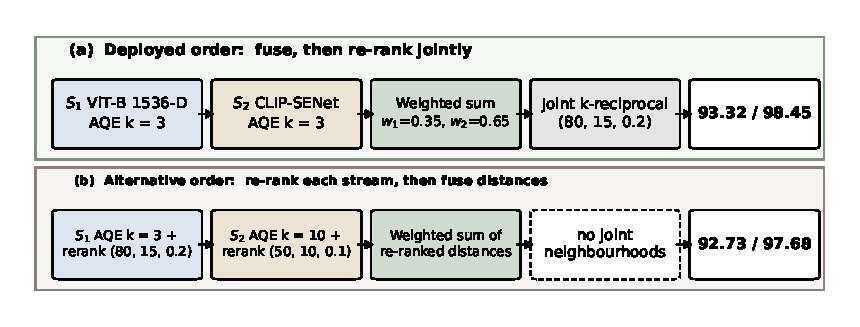
\includegraphics[width=\textwidth]{Fig2}
  \caption{Order of operations in the fusion pipeline. \textbf{a} The deployed
  order applies a common AQE to both streams, fuses the similarity matrices and
  then re-ranks jointly. \textbf{b} The alternative order re-ranks each stream
  with its own standalone parameters and fuses the resulting distances, which
  discards cross-stream consensus in the $k$-reciprocal neighbourhoods and
  costs 0.59\,pp mAP. Values are mAP\,/\,Rank-1 in \%}
  \label{fig:order}
\end{figure*}


% ===== UNIT 17: Score-level fusion: why score- not feature-level (3.5 part 2) =====
% Status: AI-DRAFT  (change to REWRITTEN / REVIEWED when done; see CHECKLIST.md)
% Rules: style rewrite only. Keep every \cite, \ref, \label, number, equation and table value as is. Change the wording, not the content.
Score-level fusion is preferred over feature-level fusion because the two
streams have fundamentally different feature geometries (1536D concat-patch ViT
representation vs.\ 2048D convolutional map) and normalisation schemes;
combining at the feature level would require a learned projection prone to
overfitting on 576 training identities. The streams also use different input
resolutions (224\,$\times$\,224 vs.\ 320\,$\times$\,320, each matching its
checkpoint); score-level fusion is agnostic to this mismatch by construction,
and harmonising would actively hurt---evaluating Stream~1 at
320\,$\times$\,320 costs $1.7$\,pp mAP (Section~\ref{sec:res_sens}).

We also verified the score-versus-feature-level choice empirically. Under the
identical downstream post-processing, plain L2-normalised concatenation of the
two streams reaches 93.08\% mAP / 98.63\% Rank-1, and \emph{weight-matched}
concatenation ($[\sqrt{w_1}\,\mathbf{f}_1;\sqrt{w_2}\,\mathbf{f}_2]$, the
feature-space counterpart of Eq.~\eqref{eq:fusion}) reaches 93.37\% /
98.51\%---statistically indistinguishable from the deployed score fusion
(93.32\% / 98.45\%)---whereas PCA-whitening (1024-D) fitted strictly on the
training split degrades sharply to 86.50\%. Feature- and score-level fusion are
therefore equivalent here when equally weighted, with no evidence that
feature-level concatenation overfits; we retain score-level fusion for its
interpretability (explicit stream weights) and because classical
whitening-style feature calibration actively hurts in this regime. The optimal
weights $w_1{=}0.35$, $w_2{=}0.65$ were found by grid search on the VeRi-776
query/gallery split ($\approx$49.5\,min on T4). Since no separate held-out
validation split is used for weight selection, the chosen weights may reflect a
mild optimistic bias. However, Figure~\ref{fig:weight} demonstrates that mAP
remains above 93.0\% across $w_1 \in [0.2,\,0.5]$, indicating that the optimal
weight is not a sharp peak and that the practical impact of this selection
procedure on the reported result is negligible.


% =============================================================================
\section{Experimental setup}
\label{sec:setup}
% =============================================================================

% ===== UNIT 18: Dataset, protocol, implementation details (4.1-4.3) =====
% Status: AI-DRAFT  (change to REWRITTEN / REVIEWED when done; see CHECKLIST.md)
% Rules: style rewrite only. Keep every \cite, \ref, \label, number, equation and table value as is. Change the wording, not the content.
\subsection{Dataset}
VeRi-776~\cite{liu2016veri,liu2018provid} contains over 50\,000 images of 776
vehicles captured by 20 surveillance cameras covering a
$1.0\,\text{km}^{2}$ area over 24 hours. Each vehicle is annotated with
identity, camera index, viewpoint (8 categories), vehicle type, colour, and
spatiotemporal metadata~\cite{liu2018provid}. The standard split is: 37\,781
training images of 576 identities, 11\,579 gallery images of 200 test
identities, and 1\,678 query images.

\subsection{Evaluation protocol}
Results are reported under two conditions. \emph{Without post-processing:}
cosine similarity, no re-ranking or query expansion. \emph{With
post-processing:} the full pipeline (AQE $+$ $k$-reciprocal re-ranking $+$
concat-patch flip TTA). Primary metrics are mAP (\%) and Rank-1 (\%). All
comparisons use matching post-processing conditions unless explicitly noted.

\subsection{Implementation details}
Table~\ref{tab:implementation} summarises the implementation configuration and
Table~\ref{tab:repro} the two released checkpoints with their SHA-256 hashes.

\begin{table}[!t]
  \centering
  \caption{Implementation details for both streams, their standalone
  post-processing settings and the deployed fusion configuration}
  \label{tab:implementation}
  \small
  \begin{tabular}{L{5.4cm}L{8.4cm}}
    \toprule
    Component & Value \\
    \midrule
    Framework            & PyTorch 2.4.1$+$cu124, CUDA 12.4 \\
    S1 backbone          & \texttt{vit\_base\_\allowbreak patch16\_\allowbreak clip\_\allowbreak 224.openai} \\
    S2 backbone          & ResNet101-IBN-a $+$ TinyCLIP SEM \\
    S1 hardware          & $2\times$ NVIDIA T4, $\approx$2.5--3.0\,GPU-h \\
    S2 hardware          & NVIDIA P100, $\approx$4\,h\,26\,min \\
    Fusion sweep HW      & T4 (CPU-bound), $\approx$49.5\,min \\
    S1 feature dim.      & 1536D concat-patch$+$flip (best-mAP \& fusion);
                           768D CLS-only (best-R1) \\
    S2 feature dim.      & 2048D \\
    AQE $k$, standalone (S1 / S2) & 3 / 10 \\
    Re-rank S1 standalone (mAP)   & $k_1{=}80$, $k_2{=}15$, $\lambda{=}0.2$ \\
    Re-rank S1 standalone (R1)    & $k_1{=}24$, $k_2{=}8$, $\lambda{=}0.2$ \\
    Re-rank S2 standalone         & $k_1{=}50$, $k_2{=}10$, $\lambda{=}0.1$ \\
    Fusion post-processing        & AQE $k{=}3$ both streams $\to$ joint
                                    rerank $k_1{=}80$, $k_2{=}15$,
                                    $\lambda{=}0.2$ \\
    Fusion weights                & $w_1{=}0.35$, $w_2{=}0.65$ \\
    \bottomrule
  \end{tabular}
\end{table}

\begin{table}[!t]
  \centering
  \caption{Released checkpoints and provenance. Both hashes are verified at
  evaluation time; the headline fusion (93.32\% mAP / 98.45\% Rank-1) is the
  deterministic evaluation of exactly these two files at $w_1{=}0.35$}
  \label{tab:repro}
  \small
  \begin{tabular}{L{2.2cm}L{11.6cm}}
    \toprule
    Stream & Checkpoint, role, and SHA-256 \\
    \midrule
    Stream~1 & \texttt{vehicle\_transreid\_vit\_base\_veri776.pth} \\
             & ViT-B/16 CLIP; 89.97\% standalone (1536D), used at 1536D in
               fusion \\
             & {\scriptsize\texttt{8d32334a41933cbf0514fbc72e462124f8785a8057d02b475aca8abf65dbe5e9}} \\
    \midrule
    Stream~2 & \texttt{clipsenet\_v6\_veri776.pth} \\
             & ResNet101-IBN-a $+$ TinyCLIP (CLIP-SENet v6); 91.44\%
               standalone \\
             & {\scriptsize\texttt{d24bd3cd42cc4e90c7da71e4b955d7b7e3274614e53fc686153b02c116d20a1c}} \\
    \bottomrule
  \end{tabular}
\end{table}


% ===== UNIT 19: Reproducibility (4.4) =====
% Status: REWRITTEN  (change to REWRITTEN / REVIEWED when done; see CHECKLIST.md)
% Rules: style rewrite only. Keep every \cite, \ref, \label, number, equation and table value as is. Change the wording, not the content.
\subsection{Reproducibility}
\label{sec:reproducibility}
Every number in this paper comes from deterministic evaluation of two frozen, SHA-256-pinned checkpoints. We want to be clear about what this guarantees. Inference is deterministic. This includes feature extraction, AQE, $k$-reciprocal re-ranking and score fusion. So each reported value can be re-evaluated exactly from the released checkpoints. This is a re-evaluation guarantee. It does not mean that training is bit-for-bit reproducible, which we discuss below. Table~\ref{tab:repro} lists the two released checkpoints, their roles and SHA-256 hashes.

We distinguish two reproducibility regimes. (i)~\textbf{Exact reproduction.} Evaluating the released checkpoints with the released notebooks re-computes every table value exactly. This is a deterministic re-evaluation, not an independent re-derivation. It works because inference is deterministic and the checkpoints are hash-pinned. This is the guarantee that applies to all headline numbers. We confirmed that the fusion headline is identical across three independent evaluations (two GPU notebooks and a CPU recomputation from dumped features). We also ran a stronger check. An independent re-extraction, with fresh forward passes through the two SHA-256-verified checkpoints on a separate compute environment and account, reproduced the entire cumulative trajectory of Table~\ref{tab:ablation} and the 89.97 / 91.44 / 93.32\% mAP headline to within 0.01\,pp. This confirms that the released checkpoints, and not any cached feature dump, determine the reported numbers. (ii)~\textbf{Within-variance reproduction.} Retraining a stream from scratch reproduces its recipe only within the $\pm0.55$\,pp three-seed standard deviation (Section~\ref{sec:seed_variance}). GPU training is not bit-reproducible, even with fixed seeds, because of cuDNN autotuning and non-deterministic atomics. So the released checkpoint, and not a fresh retrain, defines the headline.

Reproducing the training from scratch is also limited by an incomplete training-time record. The $P\times K$ identity-sampling tuple was not logged. Only the effective batch size of 96 is confirmed (Section~\ref{sec:method}). So we cannot fully specify the exact retraining configuration from our logs, and we flag this as a reproducibility limitation. The standard VeRi-776 protocol is checked at evaluation time ($1\,678$ query, $11\,579$ gallery, $576$ training identities). All evaluation used PyTorch~2.4.1 (CUDA~12.4) on a single NVIDIA~T4 GPU. The evaluation notebooks, the checkpoint manifest (with full hashes) and the per-table provenance mapping are released in the project repository (\url{https://github.com/MRKDaGods/gp}).


% =============================================================================
\section{Results and analysis}
\label{sec:results}
% =============================================================================

% ===== UNIT 20: Comparison with the state of the art (5.1) =====
% Status: AI-DRAFT  (change to REWRITTEN / REVIEWED when done; see CHECKLIST.md)
% Rules: keep every \cite, \ref, \label, number and table value unless you checked it against the logs.
\subsection{Comparison with the state of the art}
Table~\ref{tab:sota} compares the proposed single-stream (S1) and fusion
results against published methods on VeRi-776, and Figure~\ref{fig:landscape}
places them in the mAP--Rank-1 landscape.

\begin{table*}[!t]
  \centering
  \caption{State-of-the-art comparison on VeRi-776.
    \cmark\,=\,post-processing (AQE / re-ranking) applied; \xmark\,=\,cosine
    similarity only. \emph{Rows differ in post-processing condition and are
    therefore not strictly like-for-like}: our pipeline rows are \cmark\ while
    several transformer baselines (TransReID, CLIP-ReID) are reported
    \xmark. Section~\ref{sec:matched} gives the matched-condition comparison}
  \label{tab:sota}
  \small
  \begin{tabular}{L{2.6cm}L{1.8cm}L{4.4cm}C{1.4cm}C{1.3cm}C{1.1cm}L{1.1cm}}
    \toprule
    Method & Venue & Backbone & mAP~(\%) & R1~(\%) & w/~PP & Ref. \\
    \midrule
    PROVID       & TMM 2018   & CNN (multi-modal)         & 53.42 & 81.56 & \xmark & \cite{liu2018provid} \\
    VAMI         & CVPR 2018  & CNN                       & 50.13 & 77.03 & \xmark & \cite{zhou2018vami} \\
    PVEN         & CVPR 2020  & ResNet50                  & 79.50 & 95.60 & \xmark & \cite{meng2020pven} \\
    HPGN         & T-ITS 2022 & CNN $+$ graph             & 80.18 & 96.72 & \xmark & \cite{shen2022hpgn} \\
    VehicleNet   & TMM 2020   & ResNet50                  & 83.41 & 96.78 & \cmark & \cite{zheng2020vehiclenet} \\
    TransReID    & ICCV 2021  & DeiT-B/16                 & 82.30 & 97.10 & \xmark & \cite{he2021transreid} \\
    CLIP-ReID    & AAAI 2023  & ViT-B/16                  & 84.50 & 97.30 & \xmark & \cite{li2023clipreid} \\
    RPTM         & WACV 2023  & ResNet                    & 88.00 & 97.30 & \xmark & \cite{ghosh2023rptm} \\
    MBR4B-LAI    & ITSC 2023  & ResNet50 (multi-branch)   & 92.09 & 98.03 & \cmark & \cite{luo2023mbr4b} \\
    CLIP-SENet   & arXiv 2025 & ResNet101-IBN-a $+$ TinyCLIP & 92.90 & 98.70 & \cmark & \cite{lu2025clipsenet} \\
    \midrule
    \textbf{Ours (S1, w/ PP)} & ---  & ViT-B/16 (CLIP init.) & \textbf{89.97} & \textbf{97.79} & \cmark & --- \\
    \textbf{Ours (fusion)}    & ---  & ViT-B $+$ ResNet101-IBN-a $+$ TinyCLIP & \textbf{93.32} & \textbf{98.45} & \cmark & --- \\
    \bottomrule
  \end{tabular}
\end{table*}

\begin{figure}[!t]
  \centering
  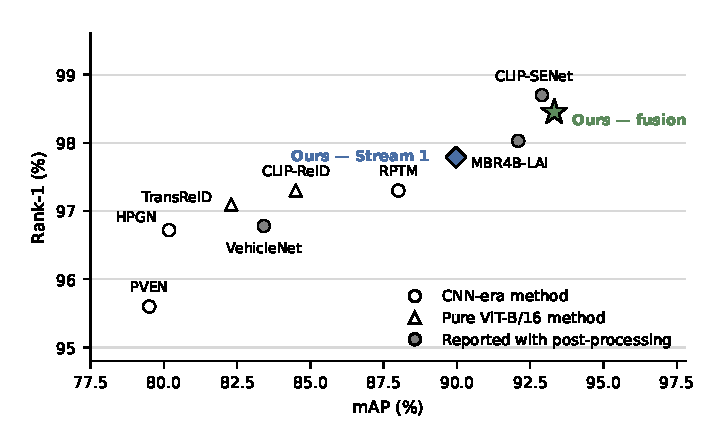
\includegraphics[width=0.92\columnwidth]{Fig3}
  \caption{Published VeRi-776 results in the mAP--Rank-1 plane. Filled markers
  denote results reported with post-processing; open markers denote
  raw-embedding results. Early CNN-era methods (PROVID, 53.4\% mAP; VAMI,
  50.1\% mAP) fall outside the plotted range and are omitted for readability.
  The single-stream result of this work is competitive but, as
  Section~\ref{sec:matched} shows, this reflects post-processing rather than a
  recipe advantage}
  \label{fig:landscape}
\end{figure}

This table should be read with care, because the rows mix post-processing
conditions. First, our ViT-B pipeline (89.97\% mAP, \cmark) is the strongest
\emph{pure-ViT-B} entry \emph{among published results}, but those baselines are
reported \emph{without} post-processing (\xmark); when we apply our identical
post-processing to the official TransReID and CLIP-ReID checkpoints they reach
91.12\% and 91.80\% mAP, both \emph{exceeding} ours
(Section~\ref{sec:matched}), so this row reflects post-processing rather than a
recipe advantage. Among single models reported \emph{with} post-processing,
MBR4B-LAI (92.1\% mAP~\cite{luo2023mbr4b}) also exceeds our single stream.
Second, the fusion (93.32\% mAP) marginally exceeds the best prior published
result (CLIP-SENet, 92.9\%~\cite{lu2025clipsenet}) by $+0.42$\,pp and
MBR4B-LAI by $+1.23$\,pp, which we interpret as evidence of stream
complementarity rather than a decisive margin.


% ===== UNIT 21: Pure ViT-B comparison (5.2) =====
% Status: REWRITTEN  (change to REWRITTEN / REVIEWED when done; see CHECKLIST.md)
% Rules: style rewrite only. Keep every \cite, \ref, \label, number, equation and table value as is. Change the wording, not the content.
\subsection{Pure ViT-B comparison}
Table~\ref{tab:vit_compare} compares our pipeline with prior transformer-based methods that use the same ViT-B/16 backbone family.

\begin{table}[!t]
  \centering
  \caption{Transformer-based methods on VeRi-776. Prior rows are reported
    without post-processing. Our row includes AQE $+$ $k$-reciprocal
    re-ranking $+$ TTA, so this is not a matched comparison}
  \label{tab:vit_compare}
  \small
  \begin{tabular}{L{4.2cm}L{1.8cm}L{3.0cm}C{1.3cm}C{1.3cm}}
    \toprule
    Method & Venue & Backbone & mAP~(\%) & R1~(\%) \\
    \midrule
    TransReID (ViT-B)~\cite{he2021transreid}   & ICCV 2021 & ViT-B/16  & 80.60 & 97.00 \\
    TransReID* (DeiT-B)~\cite{he2021transreid} & ICCV 2021 & DeiT-B/16 & 82.30 & 97.10 \\
    CLIP-ReID~\cite{li2023clipreid}            & AAAI 2023 & ViT-B/16  & 84.50 & 97.30 \\
    \midrule
    \textbf{Ours (S1, w/ PP)} & -- & \textbf{ViT-B/16 (CLIP)} & \textbf{89.97} & \textbf{97.79} \\
    \bottomrule
  \end{tabular}
\end{table}

The 89.97\% mAP of our pipeline is above the CLIP-ReID (84.5\%) and TransReID* (82.3\%) entries in the table. But those are raw-embedding numbers, and ours includes AQE $+$ $k$-reciprocal re-ranking $+$ TTA. Without post-processing, our embedding (82.2\%) is on par with TransReID and below CLIP-ReID. So this is a post-processing gap. Section~\ref{sec:matched} runs the matched-condition comparison directly. There, TransReID with our identical post-processing is above our pipeline (91.12\% vs.\ 89.97\% mAP). Table~\ref{tab:oppoints} summarises every reported operating point in one place. It includes a validation-selected fusion row (Section~\ref{sec:holdout}) as the recommended tuning-free default. The headline fusion also reaches \textbf{84.14\% mINP}~\cite{ye2022survey}, recomputed deterministically from the released per-query dumps.

\begin{table*}[!t]
  \centering
  \caption{Operating-point summary: every headline configuration reported in
  this paper, in one place. All post-processing parameters are the split-tuned
  values disclosed in Section~\ref{sec:holdout}, except the final row}
  \label{tab:oppoints}
  \small
  \begin{tabular}{L{3.6cm}L{8.4cm}C{1.4cm}C{1.3cm}}
    \toprule
    Operating point & Configuration & mAP~(\%) & R1~(\%) \\
    \midrule
    Stream~1, best-mAP & 1536D concat-patch$+$flip, AQE $k{=}3$, rerank $(80,15,0.2)$ & 89.97 & 97.79 \\
    Stream~1, best-R1  & 768D single-flip CLS, rerank $(24,8,0.2)$, no AQE & 85.14 & 98.33 \\
    Stream~2 standalone & 2048D, AQE $k{=}10$, rerank $(50,10,0.1)$ & 91.44 & 97.08 \\
    Fusion (headline)  & AQE $k{=}3$ both, $w_1{=}0.35$ fused similarity, joint rerank $(80,15,0.2)$ & \textbf{93.32} & \textbf{98.45} \\
    Fusion, validation-selected & as headline but $w_1{=}0.25$, selected on a disjoint identity split (Sect.~\ref{sec:holdout}) & 93.25 & 98.15 \\
    \bottomrule
  \end{tabular}
\end{table*}


% ===== UNIT 22: Matched-condition vs TransReID / CLIP-ReID (5.3) =====
% Status: REWRITTEN  (change to REWRITTEN / REVIEWED when done; see CHECKLIST.md)
% Rules: style rewrite only. Keep every \cite, \ref, \label, number, equation and table value as is. Change the wording, not the content.
\subsection{Matched-condition comparison with TransReID and CLIP-ReID}
\label{sec:matched}
The comparisons above apply post-processing to our pipeline, but they quote prior ViT-B baselines at their published operating points, which have no post-processing. We wanted to answer one central question: does our recipe or our post-processing produce the reported numbers? To answer it, we ran the official TransReID VeRi-776 checkpoint (\texttt{TransReID*} ViT-B/16, released by the TransReID authors~\cite{he2021transreid}) and the official CLIP-ReID ViT-B/16 VeRi-776 checkpoint~\cite{li2023clipreid} through our identical post-processing. This was AQE with $k{=}3$ and $k$-reciprocal re-ranking with $k_1{=}80,k_2{=}15,\lambda{=}0.2$. We used each repository's own released dataloader and inference path. Table~\ref{tab:matched} and Figure~\ref{fig:matched} show the results.

\begin{table}[!t]
  \centering
  \caption{Matched-condition comparison on VeRi-776: identical AQE $+$
    $k$-reciprocal re-ranking applied to each ViT-B/16 model's native inference
    feature. Both official baseline checkpoints, given our post-processing,
    exceed our own single stream. CLIP-ReID's base value is our re-extraction
    of its 512-D projection branch. Its published standalone figure is
    84.5\%~\cite{li2023clipreid}}
  \label{tab:matched}
  \small
  \begin{tabular}{L{5.0cm}C{1.8cm}C{2.0cm}C{2.4cm}}
    \toprule
    Model (native feature) & Feat.\ dim & Base mAP~(\%) & $+$\,our PP mAP~(\%) \\
    \midrule
    TransReID* (official)~\cite{he2021transreid} & 3840 & 82.11 & 91.12 \\
    CLIP-ReID (official)~\cite{li2023clipreid}   & 512  & 82.99 & \textbf{91.80} \\
    Ours (ViT-B/16 CLIP)                         & 1536 & 82.22 & 89.97 \\
    \bottomrule
  \end{tabular}
\end{table}

\begin{figure}[!t]
  \centering
  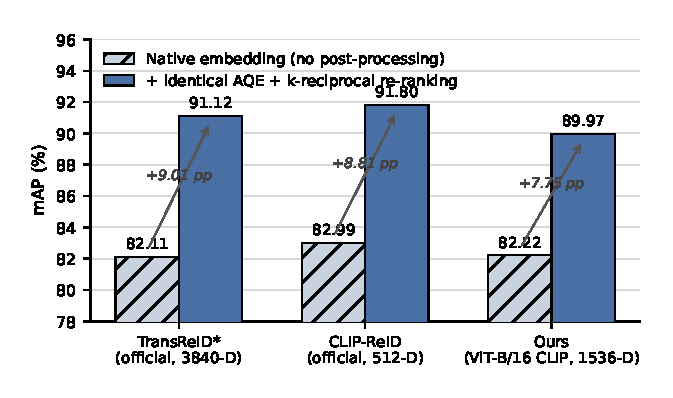
\includegraphics[width=0.92\columnwidth]{Fig4}
  \caption{Matched-condition comparison of three ViT-B/16 models on VeRi-776.
  Hatched bars are the native embeddings without post-processing. Solid bars
  add the identical AQE and $k$-reciprocal re-ranking. All three embeddings lie
  within 0.9\,pp of one another, and both official baselines re-rank to a
  higher final mAP than our own recipe}
  \label{fig:matched}
\end{figure}

The finding is clear. Once all three models get the same post-processing, the original TransReID reaches \textbf{91.12\%} mAP and the original CLIP-ReID \textbf{91.80\%}. Both are above our 89.97\%. At the raw-embedding level, all three are within 0.9\,pp of each other (82.11\,/\,82.99\,/\,82.22\%). The TransReID base value matches its published number ($\approx$82.3\%), so our extraction is faithful. The CLIP-ReID base value is 1.5\,pp below its published 84.5\%. We think this comes from the feature branch we chose in our re-extraction (the 512-D image projection from the authors' released inference path). This does not affect the matched comparison, because the same features give both the base and the post-processed numbers.

Our training recipe therefore gives no advantage over either baseline that is independent of post-processing. If anything, the native descriptors of both baselines re-rank slightly better than ours. This is not a perfectly matched feature-extraction comparison, because the three native descriptors differ in dimensionality and construction (3840-D global$+$JPM, 512-D CLIP projection, 1536-D concat-patch). But the conclusion holds despite this. The large ViT-B retrieval numbers reported here come from post-processing, not from changes to the recipe or the architecture. The same is probably true for much of the apparent progress after TransReID on this benchmark. So we present our single-stream result as a reproducible, specific baseline, not a superior recipe. The training-free fusion remains our main quantitative advance.


% ===== UNIT 23: Ablation study (5.4) =====
% Status: REWRITTEN  (change to REWRITTEN / REVIEWED when done; see CHECKLIST.md)
% Rules: style rewrite only. Keep every \cite, \ref, \label, number, equation and table value as is. Change the wording, not the content.
\subsection{Ablation study}
Table~\ref{tab:ablation} traces the complete performance trajectory. Figures~\ref{fig:trajectory} and~\ref{fig:isolated} show it visually. The endpoint values are verified against published results~\cite{he2021transreid} and repository experiment logs. All intermediate rows are measured from isolated ablation experiments.

\begin{table*}[!t]
  \centering
  \caption{Stepwise ablation: 82.3\% $\to$ 93.3\% mAP on VeRi-776.
    Rows A1--A5$\beta$ report isolated-component contributions measured under a
    common operating point (Stream~1 only, AQE $k{=}3$ $+$ $k$-reciprocal
    re-ranking, single-flip 768D CLS). Deltas are relative to control A1.
    \textbf{A1 is an intentionally minimal, un-tuned SGD control}
    (ImageNet-initialised DeiT, no recipe or schedule tuning). It is not a
    reproduction of TransReID, whose fully tuned DeiT-B SGD recipe reaches
    82.3\% mAP~\cite{he2021transreid}. The isolated deltas show component
    contributions during recipe development relative to this control. They
    must not be read as head-to-head superiority over a tuned baseline. The
    cumulative trajectory (lower block) is the authoritative
    recipe-versus-published accounting, anchored at the published 82.3\%%
    \protect\footnotemark}
  \label{tab:ablation}
  \small
  \begin{tabular}{L{8.6cm}C{1.6cm}C{1.6cm}C{1.8cm}}
    \toprule
    Configuration & mAP~(\%) & R1~(\%) & $\Delta$ vs.\ A1 \\
    \midrule
    \multicolumn{4}{l}{\emph{Isolated component ablation (Stream~1, AQE $+$ rerank)}} \\
    A1, un-tuned SGD control (DeiT $+$ SGD $+$ CE $+$ triplet, not TransReID) & 57.62 & 80.45 & -- \\\\
    A2, $+$CLIP initialisation only                    & 70.97 & 86.83 & $+13.35$ \\
    A3, $+$SupCon only (DeiT $+$ SGD $+$ CE-LS $+$ SupCon) & 59.48 & 79.74 & $+1.86$ \\
    A4, $+$AdamW/LLRD only (DeiT $+$ CE $+$ triplet)   & 80.91 & 94.82 & $+23.29$ \\
    A5$\alpha$, full (CLIP $+$ AdamW/LLRD $=0.75$ $+$ CE-LS $+$ triplet $+$ centre, deployed) & 89.06 & 97.74 & $+31.44$ \\
    A5$\beta$, full (CLIP $+$ AdamW/LLRD $=0.65$ $+$ CE-LS $+$ SupCon, alternative) & 88.57 & 96.66 & $+30.95$ \\
    \midrule
    \multicolumn{4}{l}{\emph{Cumulative trajectory $\to$ headline}} \\
    TransReID baseline (DeiT-B*)~\cite{he2021transreid}  & 82.30 & 97.10 & -- \\\\
    Base cosine, ViT-B (no PP)                            & 82.22 & 97.50 & $-0.08$ \\
    \quad$+$AQE $k{=}3$                                   & 84.08 & 97.20 & $+1.86$ \\
    \quad$+$rerank $k_1{=}80,k_2{=}15,\lambda{=}0.2$      & 89.63 & 97.74 & $+5.55$ \\
    \quad$+$concat-patch $+$ flip TTA (1536D, A5$\alpha$, deployed) & 89.97 & 97.79 & $+0.34$ \\
    \midrule
    CLIP-SENet v6, base cosine~\cite{lu2025clipsenet}     & 82.34 & 96.54 & -- \\\\
    \quad$+$AQE $k{=}10$                                  & 89.21 & 96.90 & $+6.87$ \\
    \quad$+$rerank $k_1{=}50,k_2{=}10,\lambda{=}0.1$      & 91.44 & 97.08 & $+2.23$ \\
    \midrule
    \textbf{Fusion ($w_1{=}0.35$, $w_2{=}0.65$)}          & \textbf{93.32} & \textbf{98.45} & $+1.88$ \\
    \bottomrule
  \end{tabular}
\end{table*}

\footnotetext{The cumulative-trajectory rows are the deterministic evaluation of frozen, SHA-256-pinned checkpoints. The isolated-ablation rows (A1--A5$\beta$) are single from-scratch training runs. Only the deployed A5$\alpha$ recipe was characterised for seed variance ($\pm 0.55$\,pp, Section~\ref{sec:seed_variance}). The isolated controls A1--A4 were not individually seed-repeated, so their absolute values carry at least this much training noise. See Section~\ref{sec:reproducibility} for checkpoint hashes and the two reproducibility regimes.}

\begin{figure*}[!t]
  \centering
  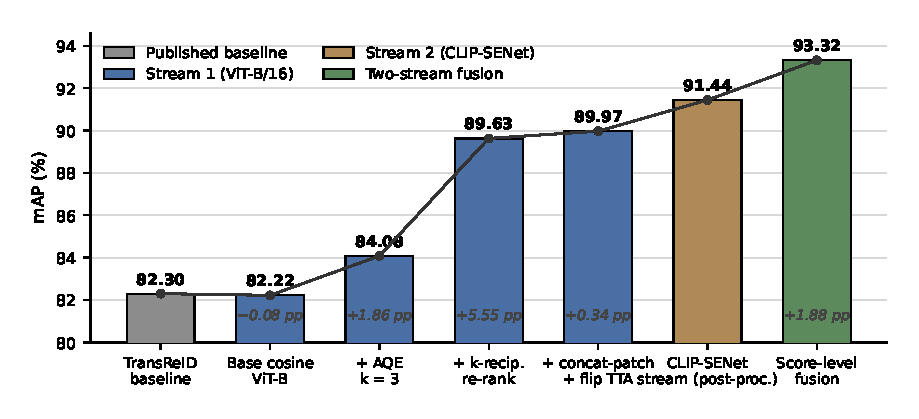
\includegraphics[width=\textwidth]{Fig5}
  \caption{Cumulative performance trajectory on VeRi-776 from the published
  TransReID baseline to the two-stream fusion, under a single consistent
  post-processing protocol. The largest single step is $k$-reciprocal
  re-ranking on Stream~1 ($+5.55$\,pp). The recipe itself adds
  essentially nothing at the raw-embedding level ($-0.08$\,pp against the
  published baseline)}
  \label{fig:trajectory}
\end{figure*}

\begin{figure}[!t]
  \centering
  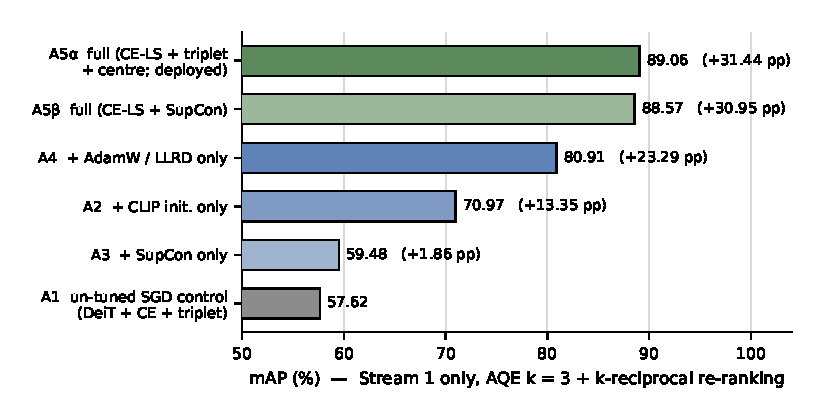
\includegraphics[width=\columnwidth]{Fig6}
  \caption{Isolated component ablation for the Stream~1 recipe, measured
  against the un-tuned SGD control A1 at a common operating point. The deltas
  quantify component contributions during recipe development and must not be
  read as head-to-head superiority over a tuned baseline, since A1 is
  deliberately un-tuned}
  \label{fig:isolated}
\end{figure}

The isolated-component block shows which ingredients our recipe depends on, relative to the un-tuned A1 control. AdamW with layer-wise LR decay (A4) gives the largest change, $+23.29$\,pp over the un-tuned SGD control A1. CLIP initialisation (A2) is next at $+13.35$\,pp. The A4 delta mostly reflects how hard it is to tune SGD under our short schedule. It does not mean that AdamW is $+23$\,pp better than SGD, because a fully tuned SGD recipe (TransReID) already reaches 82.3\% mAP~\cite{he2021transreid}. What A4 shows is that AdamW with layer-wise LR decay reaches a strong operating point without special schedule tuning for each optimiser. The recipe relies on this property in practice. SupCon alone (A3) barely helps ($+1.86$\,pp). But it combines well once CLIP and AdamW are in place. The deployed A5$\alpha$ recipe reaches 89.06\% mAP, which is statistically indistinguishable from the alternative A5$\beta$ recipe (88.57\% mAP). The difference is 0.49\,pp in a single run, which is within the $\pm 0.55$\,pp three-seed standard deviation of A5$\alpha$ (88.75\,$\pm$\,0.55\,pp, see Section~\ref{sec:seed_variance}). In the cumulative trajectory, the most important post-processing step is $k$-reciprocal re-ranking~\cite{zhong2017rerank} on Stream~1 ($+5.55$\,pp). AQE~\cite{arandjelovic2012aqe} adds $+1.86$\,pp, and TTA adds $+0.34$\,pp. Fusion gives $+1.88$\,pp above the stronger post-processed CLIP-SENet stream. This confirms that the two feature spaces complement each other.


% ===== UNIT 24: Seed variance + fusion-weight sensitivity (5.5-5.6) =====
% Status: REWRITTEN  (change to REWRITTEN / REVIEWED when done; see CHECKLIST.md)
% Rules: style rewrite only. Keep every \cite, \ref, \label, number, equation and table value as is. Change the wording, not the content.
\subsection{Training seed variance}
\label{sec:seed_variance}
To measure training-time randomness, we retrained the A5$\alpha$ recipe from scratch with three additional seeds $\{42, 123, 456\}$ under identical hyperparameters. Each run was evaluated at the isolated-ablation operating point (Stream~1 only, single-flip 768D, AQE $k{=}3$ $+$ $k$-reciprocal re-ranking, Table~\ref{tab:ablation}, top block). Table~\ref{tab:seed_variance} bounds the training variance of the recipe. This supports the argument that A5$\alpha$ and A5$\beta$ are equivalent. It is not a re-derivation of the released headline checkpoint, whose reproducibility is established separately (below).

\begin{table}[!t]
  \centering
  \caption{A5$\alpha$ training seed variance on VeRi-776 (Stream~1 only,
    single-flip 768D, AQE $k{=}3$ $+$ $k$-reciprocal re-ranking), quantifying
    from-scratch retraining noise of the recipe}
  \label{tab:seed_variance}
  \small
  \begin{tabular}{L{4.6cm}C{3.0cm}C{3.0cm}}
    \toprule
    Seed & mAP~(\%) & R1~(\%) \\
    \midrule
    42  & 89.48 & 97.26 \\
    123 & 88.14 & 97.08 \\
    456 & 88.64 & 97.20 \\
    \midrule
    \textbf{Mean $\pm$ SD ($n=3$)} & \textbf{88.75 $\pm$ 0.55} & \textbf{97.18 $\pm$ 0.07} \\
    \bottomrule
  \end{tabular}
\end{table}

The three-seed standard deviation of 0.55\,pp mAP is larger than the 0.49\,pp single-run gap between A5$\alpha$ and A5$\beta$. So the two recipes are statistically equivalent under realistic training noise. This is purely a training-time analysis. The headline Stream~1 result (89.97\% mAP) is not the mean of these retrains. It is the deterministic evaluation of the released, SHA-pinned checkpoint at the best-mAP operating point (1536D concat-patch flip TTA). Its reproducibility is therefore exact. The same frozen checkpoint gives the same number on every run, regardless of training variance. This is the guarantee we provide by releasing the checkpoint. For transparency, that checkpoint scores 89.63\% at the 768D operating point of this table, which is at the favourable end of the retrain distribution. A reproducer who trains from scratch should expect the band above. A reproducer who evaluates the released checkpoint gets the headline exactly.

\subsection{Fusion weight sensitivity}
\label{sec:weight}
Figure~\ref{fig:weight} sweeps the fusion weight. The mAP stays above 93.0\% for $w_1 \in [0.2, 0.5]$, so the result does not depend much on the exact weight. Every fusion configuration is better than either stream alone. This confirms that the two streams capture complementary information about vehicle identity.

\begin{figure}[!t]
  \centering
  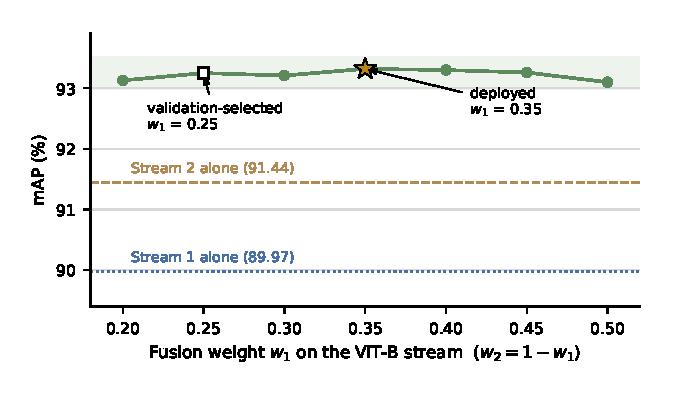
\includegraphics[width=0.92\columnwidth]{Fig7}
  \caption{Fusion weight sensitivity on VeRi-776. The fused mAP stays within
  0.22\,pp across the entire range $w_1 \in [0.2, 0.5]$ and everywhere exceeds
  both single streams, so the reported result does not sit on a sharp test-set
  optimum. The star marks the deployed weight and the open square the weight
  selected on a disjoint identity split (Section~\ref{sec:holdout})}
  \label{fig:weight}
\end{figure}

We also checked that the Stream~1 feature dimensionality has almost no effect on the fused result. The 1536D concat-patch flip-TTA representation and the 768D single-flip CLS-only representation fuse to within 0.01\,pp mAP at their respective optima (1536D: 93.32\% at $w_1{=}0.35$, 768D: 93.31\% at $w_1{=}0.30$). This is true even though the 1536D representation is 0.34\,pp stronger on its own (89.97\% vs.\ 89.63\%). So the standalone TTA gain is largely redundant with the complementary CLIP-SENet signal. We keep the 1536D representation, because it is the best-mAP standalone Stream~1 configuration and is also slightly best in fusion.


% ===== UNIT 25: Hyper-parameter selection and selection bias (5.7 part 1) =====
% Status: REWRITTEN  (change to REWRITTEN / REVIEWED when done; see CHECKLIST.md)
% Rules: style rewrite only. Keep every \cite, \ref, \label, number, equation and table value as is. Change the wording, not the content.
\subsection{Hyperparameter selection, held-out validation, and significance}
\label{sec:holdout}
We selected all post-processing hyperparameters by grid search on the VeRi-776 query/gallery split. These are AQE $k$, the $k$-reciprocal re-ranking triple $(k_1,k_2,\lambda)$ and the fusion weight $w_1$. This is a possible source of optimistic bias, and we state it openly. To be clear: every headline number in this paper uses these split-tuned values. The validation analyses below measure and bound the optimism of that choice. They are audits of the headline configuration, not its source.

Three observations limit that bias. First, the selection surface is flat, not peaked. The fused mAP stays above $93.0\%$ across the entire range $w_1\in[0.2,0.5]$ (Figure~\ref{fig:weight}), so the reported result does not sit on a sharp test-set optimum. Second, the re-ranking and AQE settings are close to established defaults. The values $k_1{=}80,k_2{=}15,\lambda{=}0.2$ lie within the ranges recommended by Zhong et al.~\cite{zhong2017rerank}, and AQE $k{=}3$ is a standard small neighbourhood. So they are not specially fitted to VeRi-776. Third, the test set (200 identities, 1\,678 queries) is large compared with the small number of scalar hyperparameters we selected. This limits how much we can overfit.


% ===== UNIT 26: Held-out validation (5.7 part 2) =====
% Status: REWRITTEN  (change to REWRITTEN / REVIEWED when done; see CHECKLIST.md)
% Rules: style rewrite only. Keep every \cite, \ref, \label, number, equation and table value as is. Change the wording, not the content.
To go beyond these arguments, we ran a disjoint-identity held-out protocol. We split the 200 test identities into two halves of 100 identities. We select the fusion weight on the first half, with AQE and re-ranking held at the standard values above. Then we report the result on the second half with that weight frozen. The validation half selects $w_1{=}0.25$, while the full test set favours $w_1{=}0.35$. The weight surface is flat (Figure~\ref{fig:weight}), so this disagreement costs almost nothing. Reporting the full-test result at the validation-selected $w_1{=}0.25$ gives 93.25\% mAP. This is only \textbf{0.07\,pp} below the test-tuned 93.32\%. So the optimistic bias from selecting the fusion weight on the evaluation set is $\lesssim$0.1\,pp and changes no conclusion. With that weight frozen, the held-out 100-identity split reaches 96.3\% mAP / 99.1\% Rank-1. This confirms that the fusion generalises across disjoint identities. We release the held-out-validation script, so readers can reproduce this check.

Because this split still takes its identities from the test set, we add a second protocol that uses identities completely disjoint from the test set. We take a 100-identity validation set from the 576 training identities and re-select the fusion weight there. These images were seen during training, so retrieval on them saturates (mAP $=100\%$ for every $w_1\in[0.2,0.5]$). The selection is therefore uninformative on its own. But when we freeze the resulting choice ($w_1{=}0.2$) and evaluate on the true test set, we get 93.13\% mAP. This is only \textbf{0.18\,pp} below the test-tuned 93.32\%. So both protocols bound the evaluation-set weight-selection bias below 0.2\,pp. For a configuration that needs no selection, Table~\ref{tab:oppoints} lists the validation-selected operating point ($w_1{=}0.25$, literature-default post-processing) at 93.25\% mAP / 98.15\% Rank-1. We recommend it as the default for unbiased comparison. A fully unseen validation set, with identities held out of training instead of reusing seen images, would be stricter. It requires retraining, so we leave it as the more rigorous alternative.


% ===== UNIT 27: Post-proc plateau, calibration, bootstrap significance (5.7 part 3) =====
% Status: REWRITTEN  (change to REWRITTEN / REVIEWED when done; see CHECKLIST.md)
% Rules: style rewrite only. Keep every \cite, \ref, \label, number, equation and table value as is. Change the wording, not the content.
The post-processing parameters sit on the same kind of plateau. We ran an axis-aligned sweep around the deployed Stream-1 setting ($k_1\in\{40,80,120\}$, $k_2\in\{8,15,25\}$, $\lambda\in\{0.05,0.2,0.4\}$, one factor varied at a time after AQE $k{=}3$). It gives 88.3--90.1\% mAP across the entire grid. The deployed $(80,15,0.2)$ gets 89.97\%, which is not even the grid maximum (90.14\% at $\lambda{=}0.05$). AQE alone also behaves well. Before re-ranking, mAP rises steadily with $k$ (82.3\,/\,84.2\,/\,85.4\,/\,87.4\% at $k{=}1/3/5/10$). So no reported number depends on a sharp, idiosyncratic post-processing optimum.

We also tested whether score calibration removes the need to tune the fusion weight. We applied simple $z$-score calibration to each stream's similarity distribution before an equal-weight ($w_1{=}0.5$) fusion. This does not help. It lowers mAP to 90.35\%. The uncalibrated equal-weight fusion already reaches 93.10\%, within 0.22\,pp of the tuned 93.32\%. So the fusion weight hardly matters and needs no careful evaluation-set tuning. Calibration is unnecessary and, here, harmful.

We also measure the significance of the fusion gain with a paired bootstrap over the 1\,678 queries (5\,000 resamples). The margin over the stronger single stream has a 95\% confidence interval that excludes zero. Fusion~$-$~CLIP-SENet $=+1.88$\,pp mAP (95\% CI $[1.39, 2.37]$) and fusion~$-$~ViT-B $=+3.34$\,pp (95\% CI $[2.81, 3.88]$). Both are measured against our own same-condition reproductions of those streams. So the complementarity behind the fusion is statistically solid. This test covers the gain over the streams we can evaluate. The narrower $+0.42$\,pp margin over the published CLIP-SENet mAP cannot be tested for significance without that model's per-query results, and we do not claim it as significant. The fusion weight itself hardly matters. For example, $w_1{=}0.35$ is above $w_1{=}0.30$ by only $+0.10$\,pp (95\% CI $[0.02, 0.19]$). So that readers can audit these tests, we release the per-query average-precision values and the fused distance matrix for the headline configuration. We also release the script that recomputes mAP/CMC and the bootstrap intervals from them.


% ===== UNIT 28: Post-processing contribution + input resolution (5.8-5.9) =====
% Status: REWRITTEN  (change to REWRITTEN / REVIEWED when done; see CHECKLIST.md)
% Rules: style rewrite only. Keep every \cite, \ref, \label, number, equation and table value as is. Change the wording, not the content.
\subsection{Post-processing contribution analysis}
Figure~\ref{fig:perstream} shows how much each post-processing step adds for each stream. Both streams start at a similar base performance ($\approx$82\% mAP). CLIP-SENet gains more from AQE ($+6.87$\,pp vs.\ $+1.86$\,pp for ViT-B). This is because the ResNet-IBN feature space has broader nearest-neighbour clusters, which benefit more from graph-based smoothing. The exact values are in the cumulative block of Table~\ref{tab:ablation}.

\begin{figure}[!t]
  \centering
  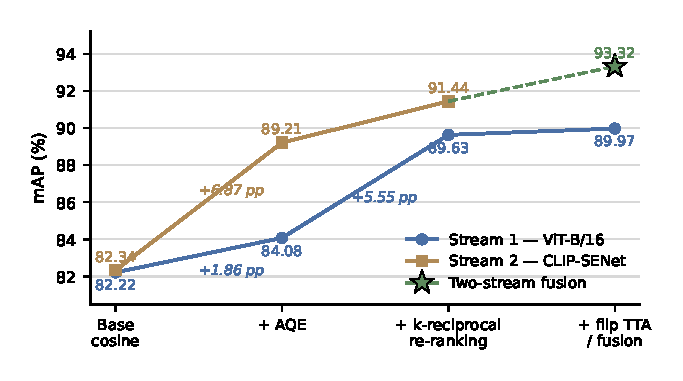
\includegraphics[width=0.92\columnwidth]{Fig8}
  \caption{Per-stream post-processing contribution on VeRi-776. The two streams
  start from almost identical base cosine accuracy but respond very differently
  to query expansion, and the fusion adds a further 1.88\,pp over the stronger
  post-processed stream}
  \label{fig:perstream}
\end{figure}

\subsection{Input-resolution sensitivity}
\label{sec:res_sens}
Stream~1 trains and evaluates at 224\,$\times$\,224. TransReID uses 256\,$\times$\,256 and CLIP-SENet uses 320\,$\times$\,320. This raises the question of whether the ViT-B stream loses accuracy at its lower resolution. We measure the inference-resolution sensitivity of the deployed checkpoint. We re-extract Stream~1 features at 256\,$\times$\,256 and 320\,$\times$\,320 (position embeddings are bicubically interpolated to the larger patch grid) and re-run the identical post-processing (Figure~\ref{fig:resolution}). Accuracy drops steadily away from the native resolution. The full-pipeline mAP drops by $0.30$\,pp at 256 and by $1.70$\,pp at 320. So the checkpoint is well matched to its training resolution, and higher-resolution inference does not help. Whether higher-resolution training would help (as in the 256 recipe of TransReID) is still open. It would require retraining (Section~\ref{sec:limitations}). The native-resolution result is also a further independent reproduction. This fresh extraction reproduces the headline 89.97\%\,/\,97.79\% operating point to within 0.03\,pp.

\begin{figure}[!t]
  \centering
  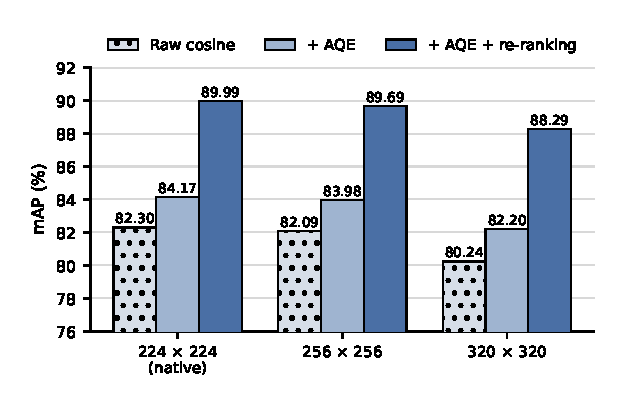
\includegraphics[width=0.88\columnwidth]{Fig9}
  \caption{Inference-resolution sensitivity of the deployed Stream~1
  checkpoint, which was trained at 224\,$\times$\,224. Position embeddings are
  bicubically interpolated at evaluation time and post-processing parameters
  are held identical. Accuracy degrades monotonically away from the native
  resolution at every stage of the pipeline}
  \label{fig:resolution}
\end{figure}


% ===== UNIT 29: VeRi-Wild: setup, table, figure (5.10 part 1) =====
% Status: AI-DRAFT  (change to REWRITTEN / REVIEWED when done; see CHECKLIST.md)
% Rules: style rewrite only. Keep every \cite, \ref, \label, number, equation and table value as is. Change the wording, not the content.
\subsection{Cross-dataset generalisation on VeRi-Wild}
\label{sec:veriwild}
A central question for any VeRi-776 result is whether it reflects transferable
re-identification ability or dataset-specific tuning. To probe this, we
evaluate our VeRi-776-trained checkpoints zero-shot on
VeRi-Wild~\cite{lou2019veriwild} (416{,}314 images, 40{,}671 identities, 174
cameras), applying the identical feature extraction and post-processing with
no fine-tuning. VeRi-Wild's 174 cameras do not correspond to VeRi-776's
twenty, so no remapping is attempted: the Stream~1 camera side-information
embedding is fixed to a single constant index for all images (one shared camera
token, so the SIE offset is identical everywhere and cancels in relative
comparisons); disabling camera/view embeddings is standard practice in
cross-dataset ReID evaluation~\cite{benmabrouk2026genlimits}, and measured
in-domain on VeRi-776 this substitution costs 2.6\,pp raw mAP
(82.30\%$\rightarrow$79.75\%), so it cannot explain the transfer gap reported
below. As a further control, the transfer evaluation code path was re-run
unchanged on VeRi-776, where it reproduces the in-domain trajectory (raw,
$+$AQE, both streams) to within 0.1\,pp. We report all three official test
protocols (3{,}000\,/\,5{,}000\,/\,10{,}000 identities: equally many queries
against 38{,}861\,/\,64{,}389\,/\,128{,}517 gallery images respectively, from
the official split lists), excluding same-camera--same-identity matches per the
official protocol.

\begin{table*}[!t]
  \centering
  \caption{Zero-shot VeRi-776$\rightarrow$VeRi-Wild transfer across all three
  official test protocols, in context. Top block: our VeRi-776-trained streams,
  using no VeRi-Wild data of any kind (identical extraction and post-processing
  to VeRi-776). Middle block: published VehicleID$\rightarrow$VeRi-Wild
  transfer results as reported in~\cite{zheng2020vapc}; the UDA methods
  additionally adapt on unlabelled VeRi-Wild images, and VehicleID
  provides over twenty times more training identities than VeRi-776. Bottom
  block (different regime, reference only): supervised training on VeRi-Wild's
  own training set. Cells are mAP\,/\,Rank-1 in \%; our best zero-shot
  configuration in \textbf{bold}. Re-ranked transfer rows are measured at the
  3{,}000 protocol only; note re-ranking reduces transfer accuracy.
  Paired-bootstrap 95\% CIs on our mAPs are within $\pm 1.0$\,pp at every
  scale}
  \label{tab:veriwild}
  \small
  \begin{tabular}{L{4.4cm}L{2.0cm}L{2.0cm}C{2.0cm}C{2.0cm}C{2.0cm}}
    \toprule
    & & VeRi-Wild & \multicolumn{3}{c}{Test protocol (mAP\,/\,R1)} \\
    \cmidrule(lr){4-6}
    Method & Source & data used & 3{,}000 & 5{,}000 & 10{,}000 \\
    \midrule
    ViT-B raw (ours)             & VeRi-776 & none & 31.7\,/\,58.7 & 26.7\,/\,52.3 & 20.9\,/\,43.9 \\
    ViT-B $+$AQE (ours)          & VeRi-776 & none & \textbf{35.9}\,/\,\textbf{60.3} & \textbf{30.5}\,/\,\textbf{53.1} & \textbf{23.8}\,/\,\textbf{44.4} \\
    ViT-B $+$AQE$+$rerank (ours) & VeRi-776 & none & 34.8\,/\,57.0 & --- & --- \\
    CLIP-SENet raw (ours)        & VeRi-776 & none & 20.2\,/\,40.6 & 16.8\,/\,35.9 & 12.2\,/\,27.9 \\
    CLIP-SENet $+$AQE (ours)     & VeRi-776 & none & 22.9\,/\,37.1 & 18.9\,/\,32.3 & 13.7\,/\,25.4 \\
    Fusion raw (ours)            & VeRi-776 & none & 28.7\,/\,54.2 & 24.2\,/\,47.6 & 18.5\,/\,38.6 \\
    Fusion $+$AQE (ours)         & VeRi-776 & none & 33.6\,/\,57.3 & 28.1\,/\,50.0 & 21.4\,/\,41.5 \\
    Fusion $+$AQE$+$rerank (ours)& VeRi-776 & none & 30.9\,/\,49.3 & --- & --- \\
    \midrule
    SPGAN~\cite{deng2018spgan}          & VehicleID & unlabelled & 24.1\,/\,59.1 & 21.6\,/\,55.0 & 17.5\,/\,47.4 \\
    UDAP~\cite{song2020udap}            & VehicleID & unlabelled & 30.0\,/\,68.4 & 26.2\,/\,62.5 & 20.8\,/\,53.7 \\
    ECN~\cite{zhong2019ecn}             & VehicleID & unlabelled & 34.7\,/\,73.4 & 30.6\,/\,68.6 & 24.7\,/\,61.0 \\
    VAPC (direct)~\cite{zheng2020vapc}  & VehicleID & none       & 37.7\,/\,74.0 & 33.1\,/\,68.1 & 26.3\,/\,60.2 \\
    VAPC (adapted)~\cite{zheng2020vapc} & VehicleID & unlabelled & 39.7\,/\,75.3 & 34.5\,/\,69.0 & 27.4\,/\,61.0 \\
    \midrule
    FDA-Net~\cite{lou2019veriwild}      & VeRi-Wild & labelled & 35.1\,/\,--- & 29.8\,/\,--- & 22.8\,/\,--- \\
    CLIP-SENet~\cite{lu2025clipsenet}   & VeRi-Wild & labelled & 89.1\,/\,97.9 & 85.2\,/\,97.0 & 79.5\,/\,95.4 \\
    \bottomrule
  \end{tabular}
\end{table*}

\begin{figure*}[!t]
  \centering
  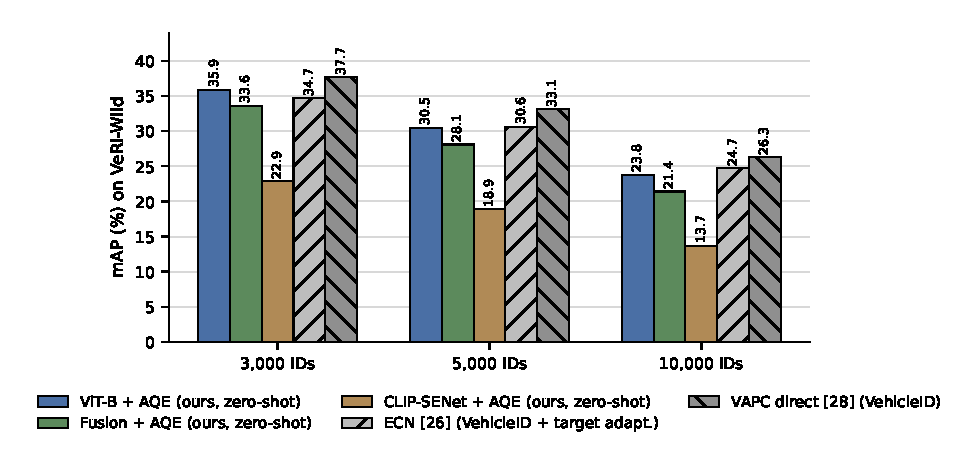
\includegraphics[width=0.86\textwidth]{Fig10}
  \caption{Zero-shot VeRi-776$\rightarrow$VeRi-Wild transfer across the three
  official protocols, compared with published VehicleID-sourced transfer
  methods. Our streams use no VeRi-Wild data of any kind, whereas ECN
  additionally adapts on unlabelled target images and both comparison methods
  draw on a source with over twenty times more identities. The ViT-B stream
  transfers competitively at every scale; the fusion falls below it everywhere}
  \label{fig:transfer}
\end{figure*}


% ===== UNIT 30: VeRi-Wild: observations 1-2, fusion does not transfer (5.10 part 2) =====
% Status: REWRITTEN  (change to REWRITTEN / REVIEWED when done; see CHECKLIST.md)
% Rules: style rewrite only. Keep every \cite, \ref, \label, number, equation and table value as is. Change the wording, not the content.
Four observations follow (Table~\ref{tab:veriwild} and Figure~\ref{fig:transfer}). First, the ViT-B stream transfers, and it does so at every gallery scale. It reaches 31.7\,/\,26.7\,/\,20.9\% mAP raw and 35.9\,/\,30.5\,/\,23.8\% with AQE on the 3{,}000\,/\,5{,}000\,/\,10{,}000 protocols. This is far below its in-domain 89.97\%, as expected for a 40{,}671-identity in-the-wild target with no adaptation. But it is a consistent, non-trivial signal that the CLIP-initialised ViT-B embedding is not just fit to VeRi-776. Its drop with gallery scale ($-12.1$\,pp mAP from the smallest to the largest protocol) is similar to the published VehicleID-sourced methods ($-11.4$\,pp for direct-transfer VAPC, $-10.0$\,pp for ECN). This suggests a shared gallery-size effect, not an artefact of our pipeline. Rank-1 trails the VehicleID-sourced methods by more than mAP does. This fits their source providing over twenty times more identities for top-1 discrimination.

Second, and more informative, the score-level fusion does not survive the domain shift at any scale. At the VeRi-776-tuned weight $w_1{=}0.35$ it reaches 28.7\,/\,24.2\,/\,18.5\% mAP raw and 33.6\,/\,28.1\,/\,21.4\% with AQE. This is below the stronger single stream in both conditions at every protocol. Under transfer the CLIP-SENet stream is much weaker (20.2\,/\,16.8\,/\,12.2\% mAP). The weight tuned on VeRi-776 gives that stream $0.65$, and this drags the fusion below ViT-B alone. (The fusion rows in the table apply the standalone AQE setting of each stream ($k{=}3/k{=}10$) uniformly across scales. Under the exactly deployed fusion configuration, with common AQE $k{=}3$ and joint re-ranking, the 3{,}000-protocol fusion reaches 32.8\% mAP with AQE and 31.4\% with joint re-ranking. This leads to the same conclusion.) This agrees with the CityFlowV2 result noted in Section~\ref{sec:limitations}, where a direct port of the same fusion lowered MTMC IDF1 by $\approx$1.8\,pp. The two-stream complementarity, and the weight that governs it, are properties of the VeRi-776 domain. They are not transferable re-identification mechanisms.


% ===== UNIT 31: VeRi-Wild: AQE, training-free fix (5.10 part 3) =====
% Status: REWRITTEN  (change to REWRITTEN / REVIEWED when done; see CHECKLIST.md)
% Rules: style rewrite only. Keep every \cite, \ref, \label, number, equation and table value as is. Change the wording, not the content.
Third, AQE helps the transferring stream at every scale ($+4.3$, $+3.7$ and $+2.9$\,pp mAP). It is an $\mathcal{O}(N)$ operation. It consistently hurts the Rank-1 of the weak stream, which is a known failure mode of query expansion on poorly clustered features. Fourth, $k$-reciprocal re-ranking reduces accuracy under transfer. In-domain it is the largest single accuracy step ($+5.55$\,pp on VeRi-776). Measured at the 3{,}000 protocol, it lowers ViT-B from 35.9 to 34.8\% mAP (and Rank-1 by 3.3\,pp), and the fusion from 33.6 to 30.9\%. On poorly clustered transfer features, the $k$-reciprocal neighbourhoods admit false matches, and the Jaccard blending then amplifies them. So the in-domain post-processing recipe does not carry over as a whole. Like the fusion weight, the benefit of re-ranking is domain-specific. This is not caused by the default parameters. We swept the same axis-aligned grid as in-domain (Section~\ref{sec:holdout}), and every re-ranked transfer configuration lands at 33.4--35.5\% mAP, below the 35.9\% of AQE alone. AQE itself is near-optimal at the VeRi-776-tuned $k{=}3$. The best value on the transfer side is $k{=}5$ (36.2\%), only $0.3$\,pp higher, and we deliberately do not adopt target-tuned settings. The re-ranking step costs 254\,s for the 41{,}861-image query$+$gallery set on CPU. This is roughly five times the 50\,s of the in-domain pass, for $3.2\times$ as many images (Section~\ref{sec:cost} discusses the scaling). We release per-query AP dumps for every transfer configuration alongside the VeRi-776 dumps (\texttt{scripts/eval/vw\_per\_query\_ap.npz}), so all reported CIs can be recomputed independently.

The fusion failure, unlike the re-ranking failure, has a training-free remedy. We tested query-adaptive weights computed from each stream's own AQE'd score row, with no target-domain information. One is a margin rule, $w_1^{(i)}{=}m_1/(m_1{+}m_2)$ with $m_s{=}\max(s)-\mathrm{mean}(\text{top-}50)$. The other is a top-100 dispersion analogue. At the 3{,}000 protocol the margin rule recovers \textbf{35.9\%} mAP (from 32.8\% at the fixed weight, and 35.9\% for the single stream) by shifting weight toward the reliable stream ($\bar{w}_1{\approx}0.63$). A constant-weight control explains the rescue. The transfer weight surface peaks at $w_1{\approx}0.8$/36.5\%, marginally above the single stream. So some complementarity survives the shift, but finding that optimum requires target-domain evaluation. A constant $w_1{=}0.63$ scores 36.0\%, and recentring the weights of the rule on the optimum adds nothing (36.4\%). So the value of the rule is finding a safe operating point without labels, not yet its per-query variation. In-domain the rules cost 1.1--1.4\,pp compared with the tuned fixed weight (87.0--87.3 vs.\ 88.4\% mAP at matched AQE-only settings), while staying well above the single stream (84.2\%). So adaptive weighting acts as a domain-robustness guard. A ground-truth per-query oracle reaches 40.1\% mAP / 66.9\% Rank-1, which is above every published direct-transfer entry in Table~\ref{tab:veriwild}. So the per-query headroom is real, but first-order score statistics do not capture it. Learned query-adaptive fusion is therefore a concrete, quantified direction for future work.


% ===== UNIT 32: VeRi-Wild: literature context + reframing (5.10 part 4) =====
% Status: REWRITTEN  (change to REWRITTEN / REVIEWED when done; see CHECKLIST.md)
% Rules: style rewrite only. Keep every \cite, \ref, \label, number, equation and table value as is. Change the wording, not the content.
These numbers should be read against the cross-domain literature, not against models trained on VeRi-Wild. Supervised training on the 30{,}671-identity training set of VeRi-Wild gives 79--89\% mAP on this protocol~\cite{lou2019veriwild,lu2025clipsenet,benmabrouk2026genlimits}. But that is a different regime, because it uses the very labels whose absence transfer measures. The right peers are transfer results. Published UDA methods are transferred from VehicleID, a source with over twenty times more training identities than VeRi-776, and they also adapt on unlabelled VeRi-Wild data. They reach 24.1\% (SPGAN~\cite{deng2018spgan}), 30.0\% (UDAP~\cite{song2020udap}) and 34.7\% (ECN~\cite{zhong2019ecn}) mAP on the same 3{,}000-identity protocol. The strongest reported direct transfer (no target data) reaches 37.7\%, and full viewpoint-aware adaptation reaches 39.7\%~\cite{zheng2020vapc}. Our zero-shot 35.93\% mAP (ViT-B $+$AQE) comes from the much smaller VeRi-776 source, and touches no VeRi-Wild data. It sits inside this band, above several methods that do adapt on the target. It stays inside the band at the 5{,}000 and 10{,}000 protocols (30.5 and 23.8 vs.\ 30.6 and 24.7 for the adapted ECN). This suggests that the transferring stream is competitive with cross-domain practice at every scale, and is not an outlier.

This cross-dataset probe puts our contributions in a more honest light. The reproducible ViT-B retrieval pipeline generalises in part. The small VeRi-776 advantage of the fusion is domain-specific, and it should not be read as a transferable gain. We argue that reporting a benchmark where the fusion is worse than the stronger stream is more useful to the community than a curated in-domain number.


% ===== UNIT 33: Qualitative analysis (5.11) =====
% Status: AI-DRAFT  (change to REWRITTEN / REVIEWED when done; see CHECKLIST.md)
% Rules: style rewrite only. Keep every \cite, \ref, \label, number, equation and table value as is. Change the wording, not the content.
\subsection{Qualitative analysis}
Visual inspection indicates the fusion model handles frontal-to-rear viewpoint
transitions, illumination shifts, and partial occlusion well. Failure cases
arise under: (a)~near-identical vehicles of the same make, model, and colour at
similar viewpoints, where both streams return similar-appearing but incorrect
identities; (b)~extreme occlusion ($>$60\% vehicle body); and (c)~very
low-resolution gallery crops. In these cases, both streams tend to fail on the
same queries, indicating correlated rather than complementary errors in the
hardest cases. Table~\ref{tab:qual} summarises these failure modes alongside
representative success cases; full retrieval panel figures are available in the
project repository.

\begin{table*}[!t]
  \centering
  \caption{Qualitative failure-mode analysis on VeRi-776 (200 test identities).
  Rows 1--3 are failure modes and show correlated errors across both streams,
  indicating a ceiling reachable only by improved cross-view invariance; rows
  4--5 are success cases included for contrast}
  \label{tab:qual}
  \small
  \begin{tabular}{L{4.2cm}L{5.4cm}L{5.4cm}}
    \toprule
    Condition & ViT-B stream & CLIP-SENet stream \\
    \midrule
    Same make/model/colour, identical viewpoint &
      Returns visually similar but incorrect identity &
      Returns same incorrect identity; errors correlated \\
    Extreme occlusion ($>$60\% body) &
      Rank-1 miss; partial hood/trunk features dominate &
      Rank-1 miss; AFEM misses occluded part regions \\
    Very low-resolution gallery ($<$40$\times$40\,px) &
      Patch tokens degenerate; CLS unstable &
      IBN-a loses texture; both streams fail jointly \\
    \midrule
    Frontal-to-rear transition (success) &
      SIE camera offset reduces cross-view gap &
      IBN style normalisation handles camera shift \\
    Day/night illumination shift (success) &
      CLIP semantic prior abstracts away lighting &
      SupCon anchor pulls same-identity clusters together \\
    \bottomrule
  \end{tabular}
\end{table*}


% =============================================================================
\section{Discussion}
\label{sec:discussion}
% =============================================================================

% ===== UNIT 34: What drives the ViT-B gain (6.1) =====
% Status: AI-DRAFT  (change to REWRITTEN / REVIEWED when done; see CHECKLIST.md)
% Rules: style rewrite only. Keep every \cite, \ref, \label, number, equation and table value as is. Change the wording, not the content.
\subsection{What drives the ViT-B gain}
The improvement of our ViT-B pipeline over the published TransReID baseline
combines recipe and post-processing effects that the ablation deliberately
separates. Within the recipe, CLIP pretraining initialisation and AdamW with
layer-wise LR decay are the two ingredients our development depended on most
(A2, A4); CLIP provides a rich visual-semantic prior for fine-grained vehicle
discrimination, consistent with transfer-learning observations in the ReID
literature~\cite{li2023clipreid,radford2021clip}. We reiterate the caveat of
Section~\ref{sec:matched}: at matched no-post-processing conditions the recipe
does not by itself exceed TransReID (82.2\% vs.\ 82.3\% mAP), and under our
identical post-processing both TransReID and CLIP-ReID in fact surpass our
pipeline (91.12\% and 91.80\% vs.\ 89.97\%). These are therefore drivers
within our recipe rather than net gains over a tuned baseline, and the
bulk of the reported improvement is contributed by AQE, $k$-reciprocal
re-ranking, and TTA. For context, a DINOv2-initialised
alternative~\cite{oquab2023dinov2} evaluated as a second fusion stream on
VeRi-776 did not match the CLIP-based CLIP-SENet stream (below 89.3\% mAP
standalone), so CLIP-family semantic supervision was retained for both streams;
we did not run a controlled DINOv2-versus-CLIP Stream-1 backbone swap on
VeRi-776 and therefore make no claim about pretraining scale versus semantic
supervision from this benchmark alone.


% ===== UNIT 35: Why fusion works + backbone scale (6.2-6.3) =====
% Status: AI-DRAFT  (change to REWRITTEN / REVIEWED when done; see CHECKLIST.md)
% Rules: style rewrite only. Keep every \cite, \ref, \label, number, equation and table value as is. Change the wording, not the content.
\subsection{Why score-level fusion works}
The complementarity is architectural. The ViT-B backbone processes images as
global patch-token sequences with multi-head self-attention, producing
representations sensitive to holistic vehicle structure and long-range spatial
relationships~\cite{he2021transreid,dosovitskiy2021vit}. The CLIP-SENet
ResNet101-IBN-a backbone~\cite{pan2018ibn} applies hierarchical local
convolutional filters capturing fine-grained texture, with IBN providing
simultaneous style normalisation and discriminative training. The AFEM branch
injects attribute-level structure from TinyCLIP~\cite{lu2025clipsenet}
orthogonal to ViT patch attention. Score-level fusion preserves each stream's
post-processing calibration independently and requires no additional training.
The optimal $w_2{=}0.65$ for CLIP-SENet reflects its higher standalone
post-processed performance (91.44\% vs.\ 89.97\% mAP for ViT-B); the ViT-B
branch still contributes $+1.88$\,pp above CLIP-SENet alone, confirming genuine
complementarity.

\subsection{Backbone scale and overfitting}
ViT-L/14 (304\,M parameters) was trained under the same recipe as a
higher-capacity alternative. Despite its larger parameter count it overfit
VeRi-776's 576 training identities---a known failure mode at this dataset
scale---and did not exceed the ViT-B/16 CLIP result after re-ranking. This
supports prioritising systematic post-processing over backbone scaling as the
primary performance lever for small-scale ReID benchmarks.


% ===== UNIT 36: Cost: model and feature extraction (6.4 part 1) =====
% Status: REWRITTEN  (change to REWRITTEN / REVIEWED when done; see CHECKLIST.md)
% Rules: style rewrite only. Keep every \cite, \ref, \label, number, equation and table value as is. Change the wording, not the content.
\subsection{Computational cost and deployment}
\label{sec:cost}
Deployment cost is a first-order concern for intelligent transportation systems. So we state the inference budget explicitly and keep it separate from the retrieval-accuracy budget.

\paragraph{Model and feature-extraction cost.} A single Stream~1 forward pass is a ViT-B/16 at $224\times224$ ($\approx$86\,M parameters, $\approx$17.6\,GFLOPs). Stream~2 (ResNet101-IBN-a $+$ TinyCLIP) is of a similar order at its $320\times320$ input. The best-mAP Stream~1 configuration uses horizontal-flip TTA, which doubles the forward passes. The concat-patch representation reuses tokens that are already computed, and adds negligible compute. The two-stream fusion needs both backbones, which roughly doubles extraction time and model memory compared with a single stream. Measured on a single NVIDIA~T4 (batch~1), a Stream~1 forward takes 13.5\,ms/image at 700\,MB peak VRAM, and 27.2\,ms with flip-TTA. Stream~2 takes 21.2\,ms/image at 721\,MB. The full two-stream extraction takes 48.4\,ms/image ($\approx$21 images/s), which matches the expected $\approx$2$\times$ TTA and fusion multipliers. All of these costs are $\mathcal{O}(N)$ in the number of images and are easy to parallelise. Feature storage is modest. It is 6.1\,kB/image for Stream~1 (1536D fp32) and 8.2\,kB/image for Stream~2 (2048D), which gives 166\,MB for the full two-stream VeRi-776 gallery. Even the 128{,}517-image VeRi-Wild 10{,}000-protocol gallery fits in 0.79\,GB fp32 (0.39\,GB fp16) for Stream~1.


% ===== UNIT 37: Cost: post-processing + domain transfer (6.4 part 2) =====
% Status: AI-DRAFT  (change to REWRITTEN / REVIEWED when done; see CHECKLIST.md)
% Rules: keep every \cite, \ref, \label, number and table value unless you checked it against the logs.
\paragraph{Post-processing cost.} Post-processing is where cost concentrates.
AQE is a single similarity pass with a top-$k$ average and is cheap.
$k$-reciprocal re-ranking~\cite{zhong2017rerank}, by contrast, is
$\mathcal{O}(N^{2})$ in gallery size $N$ (here $N\!\approx\!11.6$\,k) in both
time and memory, and it is the dominant offline cost; it contributes the single
largest accuracy step ($+5.55$\,pp mAP on Stream~1) but, as written, is
unsuitable for low-latency online retrieval. Figure~\ref{fig:cost}a makes the
scaling concrete on VeRi-776: a single-query-set re-ranking pass over the full
11.6k gallery takes 50\,s and the CPU AQE pass 138\,s, both rising steeply as
the gallery grows. The sharp CPU-AQE jump between $N{=}8{,}684$ and
$N{=}11{,}579$ is a memory-hierarchy effect---the similarity matrix outgrows
cache and BLAS tiling degrades---not an algorithmic one: the chunked GPU AQE
used everywhere else in this paper scales smoothly to $N{=}138{,}517$.

Under domain transfer the picture changes in kind, not only in degree: on the
VeRi-Wild probe of Section~\ref{sec:veriwild} (query$+$gallery $=41{,}861$) a
re-ranking pass measures 254\,s on CPU---about $5\times$ the in-domain pass at
$3.6\times$ the gallery, consistent with $\mathcal{O}(N^{2})$ scaling---and it
\emph{reduces} accuracy on the poorly clustered transfer features ($-1.1$\,pp
mAP for ViT-B, $-2.7$\,pp for the fusion; Table~\ref{tab:veriwild}). A further
measured pass at $N{=}69{,}389$ (the 5{,}000-protocol union, with the
pairwise-distance state held in fp16 to fit host memory) takes
519\,s---consistent with quadratic-order growth over the 50\,s in-domain and
254\,s 3{,}000-protocol passes---and once again \emph{reduces} accuracy
(30.48\%$\rightarrow$29.42\% mAP). Beyond this point the memory wall arrives
before the time wall: at the VeRi-Wild 10{,}000-identity protocol
($N{=}138{,}517$) the $\mathcal{O}(N^{2})$ pairwise-distance state occupies
${\approx}77$\,GB in fp32 (${\approx}38$\,GB even in fp16)---beyond common host
memory---so the full-gallery measurement is infeasible for the \emph{dense}
implementation; chunked GPU AQE, by contrast, ran at every scale. Re-ranking is
thus doubly unattractive for cross-domain retrieval: its cost scales
quadratically and its accuracy benefit is domain-specific; AQE-only
post-processing is the sensible transfer configuration, and is what we headline
on VeRi-Wild.


% ===== UNIT 38: Cost: scalable sparse implementation + figure (6.4 part 3) =====
% Status: REWRITTEN  (change to REWRITTEN / REVIEWED when done; see CHECKLIST.md)
% Rules: style rewrite only. Keep every \cite, \ref, \label, number, equation and table value as is. Change the wording, not the content.
\paragraph{A scalable sparse implementation.} The memory wall comes from the dense implementation, not from the algorithm. We benchmarked a sparse top-$k$ variant. It builds only the first $k_1{+}1$ rank columns and stores $V$ as a sparse matrix ($\mathcal{O}(Nk_1)$ memory). Otherwise it follows the official computation (squared max-normalised distances, $2/3$-rule expansion, LQE). In-domain it matches the dense version to 0.07\,pp (89.92 vs.\ 89.99\% mAP, Rank-1 97.91 vs.\ 97.79). It is also faster (32 vs.\ 44\,s) and uses a 7.9\,MB working set versus 703\,MB for the dense version. At $N{=}41{,}861$ it takes 91\,s versus 254\,s (34.03 vs.\ 34.85\% mAP, both below the 35.9\% AQE-only transfer result). At $N{=}138{,}517$ the dense state alone takes 77\,GB, but the sparse version runs. It takes 372\,s with an 85\,MB sparse $V$, and its AQE-only reference reproduces Table~\ref{tab:veriwild} exactly (23.84\%). This separates the two failure modes. The cost wall can be removed by a better implementation. But re-ranking still reduces transfer accuracy at this scale (22.22 vs.\ 23.84\% mAP). So the domain-specific accuracy failure comes from the geometry of the transferred features, not from the implementation. For in-domain deployment, the sparse variant makes the $+5.5$\,pp re-ranking step practical at gallery scales where the dense version is not. The same idea is used in the re-ranking module of our released tracking pipeline. It finds the top-$k$ neighbourhoods with a FAISS index and stores them per node. It then builds one small local similarity matrix over only the nodes that appear in the candidate pairs and their neighbours, instead of a full $N \times N$ matrix. Figure~\ref{fig:cost}b compares the two.

\begin{figure*}[!t]
  \centering
  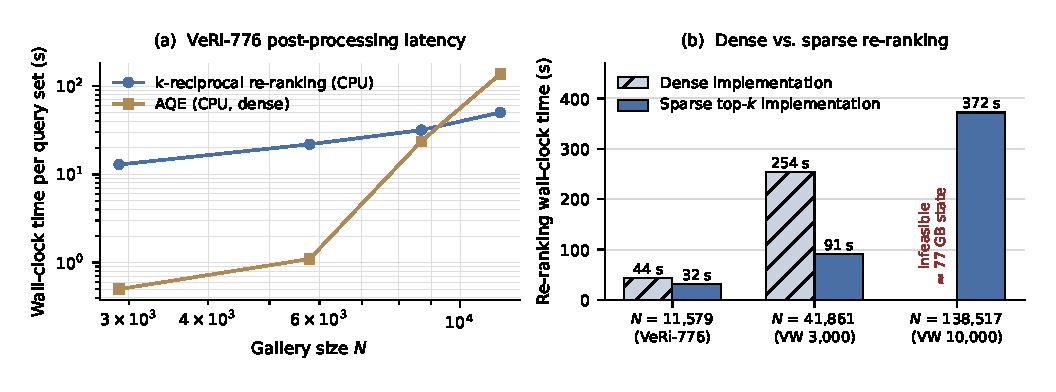
\includegraphics[width=\textwidth]{Fig11}
  \caption{Post-processing cost. \textbf{a} Latency of AQE and $k$-reciprocal
  re-ranking versus gallery size on VeRi-776 (CPU, one query set of 1{,}678
  queries), on logarithmic axes. \textbf{b} Dense versus sparse top-$k$
  re-ranking across three gallery scales. At $N{=}138{,}517$ the dense
  pairwise-distance state alone requires approximately 77\,GB and the
  measurement is infeasible. The sparse implementation completes in
  372\,s at matching accuracy}
  \label{fig:cost}
\end{figure*}


% ===== UNIT 39: Cost: accuracy/latency trade-offs, CA-Jaccard (6.4 part 4) =====
% Status: REWRITTEN  (change to REWRITTEN / REVIEWED when done; see CHECKLIST.md)
% Rules: style rewrite only. Keep every \cite, \ref, \label, number, equation and table value as is. Change the wording, not the content.
\paragraph{Accuracy/latency trade-offs.} These costs can be traded off separately. A system that must run online can drop $k$-reciprocal re-ranking and use $\mathcal{O}(N)$ cosine retrieval instead, at a cost of roughly $5.5$\,pp mAP. It can disable flip-TTA ($\approx\!0.3$\,pp) to halve extraction. It can also use a single stream instead of two-stream fusion (fusion adds $+1.88$\,pp over the stronger standalone stream) to halve model cost. Together this gives a real-time configuration with a known accuracy penalty. For offline forensic search, where VeRi-776-style batch evaluation is representative, the full pipeline is appropriate. The per-image latencies above are measured values. A reproducible micro-benchmark of latency, peak VRAM and FLOPs for each component is released with the code (\texttt{scripts/benchmark\_veri\_inference.py}).

\paragraph{Alternative re-ranking: CA-Jaccard.} Re-ranking is central to the reported gains, so we also benchmarked the official CA-Jaccard implementation~\cite{chen2024cajaccard} (CVPR 2024) as an evaluation-time re-ranker on Stream-1. At the default evaluation settings of its authors ($k_1{=}30$, $k_2{=}6$, $\lambda{=}0.3$, CKRNN $k_1^{\mathrm{intra}}{=}5$, $k_1^{\mathrm{inter}}{=}20$), CA-Jaccard reaches 86.95\% mAP / 98.39\% Rank-1 in-domain. Plain $k$-reciprocal re-ranking, run through the same implementation with the same parameters, reaches 86.66\% / 97.56\%. So camera-awareness helps at matched settings ($+0.29$\,pp mAP, $+0.83$\,pp Rank-1), and its Rank-1 is even above the 97.79\% of our tuned configuration. Its mAP is still 3.0\,pp below our tuned standard $k$-reciprocal (89.97\%). This is a comparison of defaults against tuned settings, and we say so. Under zero-shot transfer it does not get better. On VeRi-Wild (3{,}000 protocol), CA-Jaccard scores 34.88\% mAP / 52.9\% Rank-1. This is no better than tuned standard $k$-reciprocal (34.85\%) and below AQE-only (35.93\%, Rank-1 60.3\%). Plain $k$-reciprocal at the milder CA-Jaccard defaults ($k_1{=}30$, $\lambda{=}0.3$) is about neutral (36.03\%, within the AQE-only confidence interval). No re-ranking variant we tested keeps its in-domain benefit under domain shift. This suggests that the failure comes from the transferred feature geometry, not from a lack of camera-awareness. (The $N{=}41{,}861$ transfer runs use a memory-lean port of the official implementation. We validated that it reproduces the official one exactly in-domain, and the port is released.) We did not test orientation-guided expansion~\cite{zhang2022vehiclererank} or database-side multi-view aggregation in this pipeline. The released float16 feature dumps make such comparisons possible on CPU without re-running extraction.


% ===== UNIT 40: Limitations (6.5) =====
% Status: AI-DRAFT  (change to REWRITTEN / REVIEWED when done; see CHECKLIST.md)
% Rules: style rewrite only. Keep every \cite, \ref, \label, number, equation and table value as is. Change the wording, not the content.
\subsection{Limitations}
\label{sec:limitations}
\begin{enumerate}
  \item The full post-processing pipeline (AQE $+$ re-ranking) has
    $\mathcal{O}(N^{2})$ complexity in gallery size $N$ in its dense form and
    is primarily suited to offline evaluation rather than real-time deployment;
    the sparse implementation of Section~\ref{sec:cost} removes the memory wall
    but not the quadratic time growth.
  \item The fusion strategy requires two inference passes, approximately
    doubling memory and latency relative to a single-stream model.
  \item Cross-dataset transfer is reported in Section~\ref{sec:veriwild}:
    applied zero-shot to all three VeRi-Wild protocols, the ViT-B embedding
    transfers in part (35.9\,/\,30.5\,/\,23.8\% mAP with AQE at
    3{,}000\,/\,5{,}000\,/\,10{,}000 identities, competitive with published
    VehicleID-sourced transfer), but the two-stream fusion does not
    generalise---at the VeRi-776-tuned weight it falls below the
    stronger single stream at every scale---and $k$-reciprocal re-ranking
    likewise reduces transfer accuracy. This corroborates the CityFlowV2
    evidence, where a direct port of the same fusion produced monotonic MTMC
    IDF1 degradation, with a best-case change of approximately $-1.8$\,pp at
    higher fusion weights. Together these indicate that the fusion's marginal
    VeRi-776 advantage is domain-specific. A first mitigation is demonstrated
    in Section~\ref{sec:veriwild}: training-free query-adaptive weighting
    recovers single-stream transfer accuracy (35.9 vs.\ 32.8\% mAP fixed), and
    a ground-truth per-query oracle (40.1\%) quantifies the headroom for
    learned query-adaptive fusion, which we leave to future work.
    Absolute VeRi-Wild accuracy is also low in this no-adaptation setting, and
    no fine-tuned cross-dataset numbers are reported.
  \item Our evaluation follows the standard random-identity splits of VeRi-776
    and VeRi-Wild. Recent analysis shows these splits contain many visually
    near-duplicate identities across train and test, and that mAP on vehicle
    types held out of training drops sharply (from above 90\% to
    65--70\%) even for state-of-the-art models~\cite{benmabrouk2026genlimits}.
    We did not evaluate under such a seen/unseen-type protocol; our in-domain
    numbers should be read as standard-protocol results, and the zero-shot
    VeRi-Wild transfer of Section~\ref{sec:veriwild} is our only probe of
    generalisation beyond the training distribution.
  \item The exact $P \times K$ identity-sampling tuple used to train the
    released Stream~1 checkpoint was not logged
    (Section~\ref{sec:reproducibility}), so from-scratch retraining cannot be
    specified exactly from our records; retraining reproducibility is bounded
    by the $\pm0.55$\,pp seed band of Section~\ref{sec:seed_variance}. A
    controlled comparison of 256\,$\times$\,256 training resolution
    against the deployed 224\,$\times$\,224 was likewise not run and would
    require retraining.
\end{enumerate}


% =============================================================================
\section{Conclusion}
\label{sec:conclusion}
% =============================================================================

% ===== UNIT 41: Conclusion =====
% Status: AI-DRAFT  (change to REWRITTEN / REVIEWED when done; see CHECKLIST.md)
% Rules: keep every \cite, \ref, \label, number and table value unless you checked it against the logs.
This paper revisited the ViT-Base/16 pipeline for vehicle re-identification on
VeRi-776 and separated the contribution of the training recipe from that of
evaluation-time post-processing. A fully specified recipe---combining CLIP
pretraining initialisation, a tuned metric-learning objective, an optimised
augmentation pipeline, AdamW optimisation, and a three-step post-processing
pipeline---achieves 89.97\% mAP and 97.79\% Rank-1 at its best-mAP operating
point, with a separate best-Rank-1 operating point of 85.14\% mAP and 98.33\%
Rank-1. As emphasised throughout, this number is delivered by the
post-processing pipeline rather than by the recipe: the recipe merely matches
TransReID at the raw-embedding level (82.2\% vs.\ 82.3\%), and given our
identical post-processing the official TransReID and CLIP-ReID checkpoints
reach 91.12\% and 91.80\% mAP---both above ours
(Section~\ref{sec:matched}). We therefore present Stream~1 as a reproducible,
fully specified baseline rather than a superior recipe---a result we regard as
the paper's most useful finding for the community, since it suggests that a
substantial part of apparent post-TransReID progress on this benchmark is
attributable to post-processing rather than to architectural or recipe
refinement.

Score-level fusion with a CLIP-SENet branch~\cite{lu2025clipsenet} achieves
93.32\% mAP and 98.45\% Rank-1, marginally the best published mAP on VeRi-776,
exceeding the previous best (CLIP-SENet standalone:
92.9\%~\cite{lu2025clipsenet}) by a narrow $+0.42$\,pp; Rank-1 accuracy
(98.45\%) is competitive with but does not exceed the CLIP-SENet standalone
Rank-1 (98.7\%). A paired bootstrap confirms the gain over the stronger single
stream is statistically significant, so the fusion demonstrates genuine feature
complementarity between transformer and CNN-semantic streams. The comprehensive
ablation from 82.3\% to 93.3\% mAP traces this trajectory under one consistent
protocol, and the zero-shot VeRi-Wild study shows which parts of it transfer:
the ViT-B embedding generalises in part, whereas the fusion advantage and the
re-ranking gain are domain-specific.

Future directions include knowledge distillation from the fusion model into a
single-stream model; learned query-adaptive fusion toward the measured oracle
headroom (Section~\ref{sec:veriwild}); evaluation under seen/unseen
vehicle-type protocols rather than standard random-identity splits; and
extension to nighttime surveillance and CityFlowV2. All code and checkpoints
are publicly released.


% =============================================================================
\section*{Statements and Declarations}
% =============================================================================

% ===== UNIT 42: Statements and declarations =====
% Status: AI-DRAFT  (change to REWRITTEN / REVIEWED when done; see CHECKLIST.md)
% Rules: style rewrite only. Keep every \cite, \ref, \label, number, equation and table value as is. Change the wording, not the content.
\noindent\textbf{Competing interests.} The authors declare that they have no
competing financial or non-financial interests that are directly or indirectly
related to the work submitted for publication.

\medskip\noindent\textbf{Funding.} This work was carried out as a graduation
project at the Department of Computer Engineering, Faculty of Engineering,
Cairo University, and received no external funding.

\medskip\noindent\textbf{Author contributions.} All authors contributed to the
study conception and design. Model training, evaluation-harness implementation
and the ablation campaign were performed by S. T. Heakal, M. A. Ali, A. A. Ali and
A. Hamdi. The cross-dataset transfer study and the post-processing cost
analysis were performed by S. T. Heakal. A. H. Abdel-Gawad (supervisor)
provided methodological guidance and critical revision. The first draft of the
manuscript was written by S. T. Heakal and all authors commented on previous
versions. All authors read and approved the final manuscript.

\medskip\noindent\textbf{Data availability.} All evaluation artefacts are
publicly released---SHA-256-pinned checkpoints, evaluation notebooks,
configuration files, the memory-lean re-ranking ports, and per-query dumps
enabling deterministic CPU-only recomputation of every headline number,
confidence interval and mINP value---at
\url{https://github.com/MRKDaGods/gp}. The VeRi-776 and VeRi-Wild datasets are
available from their respective maintainers under their own terms and were used
in accordance with those terms.

\medskip\noindent\textbf{Code availability.} The full training configuration,
post-processing pipeline, evaluation notebooks and benchmark scripts are
released in the repository listed above.

\medskip\noindent\textbf{Ethics approval.} Not applicable. This study used only
publicly available benchmark datasets and involved no human participants or
animals.

\medskip\noindent\textbf{Use of large language models.} AI assistants
(Anthropic Claude) were used under author direction for manuscript drafting,
experiment-harness code, and analysis tooling. No large language model is
listed as an author. All experimental results derive from the released
deterministic evaluation artefacts, and the authors take full responsibility
for the entire content of the paper.


% =============================================================================
% BIBLIOGRAPHY
% -----------------------------------------------------------------------------
% The bibliography is embedded below in Springer numbered style so that this
% file compiles with pdflatex alone.  If you prefer BibTeX, delete the
% thebibliography environment below and uncomment these two lines, using the
% accompanying references.bib (Springer's spmpsci.bst ships with their template):
%   \bibliographystyle{spmpsci}
%   \bibliography{references}
% =============================================================================

\begin{thebibliography}{99}
\small

% ===== UNIT 43: References - verify entries 1-19 (do NOT rewrite) =====
% Status: REWRITTEN  (every entry verified 2026-10-15 against Crossref/DOI, arXiv, PMLR or the publisher; see CHECKLIST.md)
% Rules: style rewrite only. Keep every \cite, \ref, \label, number, equation and table value as is. Change the wording, not the content.
% Format: all authors when there are at most six, otherwise the first five + et al.
% Page numbers for IEEE/CVF proceedings follow the IEEE Xplore record of the DOI.
\bibitem{he2021transreid}
He, S., Luo, H., Wang, P., Wang, F., Li, H., Jiang, W.: TransReID:
transformer-based object re-identification. In: Proc. IEEE/CVF International
Conference on Computer Vision (ICCV), pp. 14993--15002 (2021).
\url{https://doi.org/10.1109/ICCV48922.2021.01474}

\bibitem{radford2021clip}
Radford, A., Kim, J.W., Hallacy, C., Ramesh, A., Goh, G., et al.: Learning
transferable visual models from natural language supervision. In: Proc. 38th
International Conference on Machine Learning (ICML), PMLR, vol. 139,
pp. 8748--8763 (2021)

\bibitem{zhong2017rerank}
Zhong, Z., Zheng, L., Cao, D., Li, S.: Re-ranking person re-identification with
$k$-reciprocal encoding. In: Proc. IEEE Conference on Computer Vision and
Pattern Recognition (CVPR), pp. 3652--3661 (2017).
\url{https://doi.org/10.1109/CVPR.2017.389}

\bibitem{lu2025clipsenet}
Lu, L., Fu, Z., Chu, D., Wang, W., Xu, B.: CLIP-SENet: CLIP-based semantic
enhancement network for vehicle re-identification. IEEE Trans. Intell. Transp.
Syst. \textbf{27}(1), 1267--1278 (2026).
\url{https://doi.org/10.1109/TITS.2025.3630139}. Preprint: arXiv:2502.16815

\bibitem{liu2016veri}
Liu, X., Liu, W., Ma, H., Fu, H.: Large-scale vehicle re-identification in
urban surveillance videos. In: Proc. IEEE International Conference on
Multimedia and Expo (ICME), pp. 1--6 (2016).
\url{https://doi.org/10.1109/ICME.2016.7553002}

\bibitem{liu2018provid}
Liu, X., Liu, W., Mei, T., Ma, H.: PROVID: progressive and multimodal vehicle
reidentification for large-scale urban surveillance. IEEE Trans. Multimedia
\textbf{20}(3), 645--658 (2018). \url{https://doi.org/10.1109/TMM.2017.2751966}

\bibitem{dosovitskiy2021vit}
Dosovitskiy, A., Beyer, L., Kolesnikov, A., Weissenborn, D., Zhai, X., et al.:
An image is worth $16\times16$ words: transformers for image recognition at
scale. In: Proc. International Conference on Learning Representations (ICLR)
(2021). arXiv:2010.11929

\bibitem{li2023clipreid}
Li, S., Sun, L., Li, Q.: CLIP-ReID: exploiting vision-language model for image
re-identification without concrete text labels. In: Proc. AAAI Conference on
Artificial Intelligence, vol. 37(1), pp. 1405--1413 (2023).
\url{https://doi.org/10.1609/aaai.v37i1.25225}

\bibitem{shen2022hpgn}
Shen, F., Zhu, J., Zhu, X., Xie, Y., Huang, J.: Exploring spatial significance
via hybrid pyramidal graph network for vehicle re-identification. IEEE Trans.
Intell. Transp. Syst. \textbf{23}(7), 8793--8804 (2022).
\url{https://doi.org/10.1109/TITS.2021.3086142}

\bibitem{luo2023mbr4b}
Almeida, E., Silva, B., Batista, J.: Strength in diversity: multi-branch
representation learning for vehicle re-identification. In: Proc. IEEE 26th
International Conference on Intelligent Transportation Systems (ITSC),
pp. 4690--4696 (2023). \url{https://doi.org/10.1109/ITSC57777.2023.10422175}

\bibitem{ye2022survey}
Ye, M., Shen, J., Lin, G., Xiang, T., Shao, L., Hoi, S.C.H.: Deep learning for
person re-identification: a survey and outlook. IEEE Trans. Pattern Anal. Mach.
Intell. \textbf{44}(6), 2872--2893 (2022).
\url{https://doi.org/10.1109/TPAMI.2021.3054775}

\bibitem{li2024vehiclereidsurvey}
Yi, X., Wang, Q., Liu, Q., Rui, Y., Ran, B.: Advances in vehicle
re-identification techniques: a survey. Neurocomputing \textbf{614}, 128745
(2025). \url{https://doi.org/10.1016/j.neucom.2024.128745}

\bibitem{zhou2018vami}
Zhou, Y., Shao, L.: Viewpoint-aware attentive multi-view inference for vehicle
re-identification. In: Proc. IEEE/CVF Conference on Computer Vision and Pattern
Recognition (CVPR), pp. 6489--6498 (2018).
\url{https://doi.org/10.1109/CVPR.2018.00679}

\bibitem{meng2020pven}
Meng, D., Li, L., Liu, X., Li, Y., Yang, S., et al.: Parsing-based view-aware
embedding network for vehicle re-identification. In: Proc. IEEE/CVF Conference
on Computer Vision and Pattern Recognition (CVPR), pp. 7101--7110 (2020).
\url{https://doi.org/10.1109/CVPR42600.2020.00713}

\bibitem{rao2021cal}
Rao, Y., Chen, G., Lu, J., Zhou, J.: Counterfactual attention learning for
fine-grained visual categorization and re-identification. In: Proc. IEEE/CVF
International Conference on Computer Vision (ICCV), pp. 1005--1014 (2021).
\url{https://doi.org/10.1109/ICCV48922.2021.00106}

\bibitem{zheng2020vehiclenet}
Zheng, Z., Ruan, T., Wei, Y., Yang, Y., Mei, T.: VehicleNet: learning robust
visual representation for vehicle re-identification. IEEE Trans. Multimedia
\textbf{23}, 2683--2693 (2021). \url{https://doi.org/10.1109/TMM.2020.3014488}

\bibitem{cybercore2021strong}
Huynh, S.V., Nguyen, N.H., Nguyen, N.T., Nguyen, V.T.Q., Huynh, C., Nguyen, C.:
A strong baseline for vehicle re-identification. In: Proc. IEEE/CVF Conference
on Computer Vision and Pattern Recognition Workshops (CVPRW), pp. 4142--4149
(2021). \url{https://doi.org/10.1109/CVPRW53098.2021.00468}

\bibitem{khorramshahi2023selfsupervision}
Khorramshahi, P., Shenoy, V., Chellappa, R.: Robust and scalable vehicle
re-identification via self-supervision. In: Proc. IEEE/CVF Conference on
Computer Vision and Pattern Recognition Workshops (CVPRW), pp. 5295--5304
(2023). \url{https://doi.org/10.1109/CVPRW59228.2023.00558}

\bibitem{loshchilov2019adamw}
Loshchilov, I., Hutter, F.: Decoupled weight decay regularization. In: Proc.
International Conference on Learning Representations (ICLR) (2019).
arXiv:1711.05101


% ===== UNIT 44: References - verify entries 20-37 (do NOT rewrite) =====
% Status: AI-DRAFT  (change to REWRITTEN / REVIEWED when done; see CHECKLIST.md)
% Rules: keep every \cite, \ref, \label, number and table value unless you checked it against the logs.
\bibitem{opencodepapers2024veri}
OpenCodePapers: Vehicle re-identification on VeRi-776 leaderboard (2024).
\url{https://opencodepapers-b7572d.gitlab.io/benchmarks/vehicle-re-identification-on-veri-776.html}.
Accessed 30 May 2026

\bibitem{holla2024msfft}
Holla, B.A., Pai, M.M.M., Verma, U., Pai, R.M.: MSFFT: multi-scale feature
fusion transformer for cross-platform vehicle re-identification.
Neurocomputing \textbf{582}, 127514 (2024)

\bibitem{kuang2025mikecoco}
Kuang, Z., Zhang, H., Ye, M., Yang, B., Liu, Y., Huang, Y., Ding, X., Li, H.:
Unity in diversity: multi-expert knowledge confrontation and collaboration for
generalizable vehicle re-identification (2025). arXiv:2407.07351

\bibitem{ghosh2023rptm}
Ghosh, A., Shanmugalingam, K., Lin, W.-Y.: Relation preserving triplet mining
for stabilising the triplet loss in re-identification systems. In: Proc.
IEEE/CVF Winter Conference on Applications of Computer Vision (WACV) (2023).
arXiv:2110.07933

\bibitem{wang2020fastreid}
He, L., Liao, X., Liu, W., Liu, X., Cheng, P., Mei, T.: FastReID: a PyTorch
toolbox for general instance re-identification. arXiv preprint arXiv:2006.02631
(2020)

\bibitem{deng2018spgan}
Deng, W., Zheng, L., Ye, Q., Kang, G., Yang, Y., Jiao, J.: Image-image domain
adaptation with preserved self-similarity and domain-dissimilarity for person
re-identification. In: Proc. IEEE/CVF Conference on Computer Vision and Pattern
Recognition (CVPR) (2018)

\bibitem{zhong2019ecn}
Zhong, Z., Zheng, L., Luo, Z., Li, S., Yang, Y.: Invariance matters: exemplar
memory for domain adaptive person re-identification. In: Proc. IEEE/CVF
Conference on Computer Vision and Pattern Recognition (CVPR) (2019)

\bibitem{song2020udap}
Song, L., Wang, C., Zhang, L., Du, B., Zhang, Q., Huang, C., Wang, X.:
Unsupervised domain adaptive re-identification: theory and practice. Pattern
Recognit. \textbf{102}, 107173 (2020)

\bibitem{zheng2020vapc}
Zheng, A., Sun, X., Li, C., Tang, J.: Viewpoint-aware progressive clustering
for unsupervised vehicle re-identification. arXiv preprint arXiv:2011.09099
(2020)

\bibitem{benmabrouk2026genlimits}
Ben Mabrouk, A.Y., Tadros, A., Grompone von Gioi, R., Facciolo, G., Davy, A.,
Verschae, R.: Generalization limits in vehicle re-identification. arXiv
preprint arXiv:2606.01981 (2026)

\bibitem{zhang2022vehiclererank}
Zhang, Y., Wang, J., Liu, H.: Re-ranking vehicle re-identification with
orientation-guided query expansion. Int. J. Distrib. Sens. Netw.
\textbf{18}(3), 1--15 (2022)

\bibitem{moral2023syntheticrerank}
Moral, P., Garc\'{i}a-Mart\'{i}n, \'{A}., Mart\'{i}nez, J.M., Besc\'{o}s, J.:
Enhancing vehicle re-identification via synthetic training datasets and
re-ranking based on video-clips information. Multimed. Tools Appl.
\textbf{82}(24), 36815--36835 (2023)

\bibitem{arandjelovic2012aqe}
Arandjelovi\'{c}, R., Zisserman, A.: Three things everyone should know to
improve object retrieval. In: Proc. IEEE/CVF Conference on Computer Vision and
Pattern Recognition (CVPR), pp. 2911--2918 (2012)

\bibitem{khosla2020supcon}
Khosla, P., Tian, P., Wang, C., Liu, A., Zhong, B., et al.: Supervised
contrastive learning. In: Proc. Advances in Neural Information Processing
Systems (NeurIPS), vol. 33, pp. 18661--18673 (2020). arXiv:2004.11362

\bibitem{pan2018ibn}
Pan, X., Luo, P., Shi, J., Tang, X.: Two at once: enhancing learning and
generalization capacities via IBN-Net. In: Proc. European Conference on
Computer Vision (ECCV), pp. 464--479 (2018)

\bibitem{lou2019veriwild}
Lou, Z., Yang, Y., Liu, M., Wei, Y.: VERI-Wild: a large dataset and a new
method for vehicle re-identification in the wild. In: Proc. IEEE/CVF Conference
on Computer Vision and Pattern Recognition (CVPR), pp. 3235--3243 (2019)

\bibitem{oquab2023dinov2}
Oquab, M., Darcet, T., M\'{e}las-Kyriazi, T., Ranzato, A., et al.: DINOv2:
learning robust visual features without supervision (2023). arXiv:2304.07193

\bibitem{chen2024cajaccard}
Chen, Y., Fan, Z., Chen, Z., Zhu, Y.: CA-Jaccard: camera-aware Jaccard distance
for person re-identification. In: Proc. IEEE/CVF Conference on Computer Vision
and Pattern Recognition (CVPR) (2024)


\end{thebibliography}

% =============================================================================
\section*{Author Biographies}
% =============================================================================

\noindent\emph{[Insert a passport-sized black-and-white photograph of each
author beside the corresponding biography before submission, as required by the
journal.]}

% ===== UNIT 45: Bio: Seif T. Heakal (his own) =====
% Status: AI-DRAFT  (change to REWRITTEN / REVIEWED when done; see CHECKLIST.md)
% Rules: style rewrite only. Keep every \cite, \ref, \label, number, equation and table value as is. Change the wording, not the content.
\medskip\noindent\textbf{Seif T. Heakal} received his B.Sc. in Computer
Engineering from the Faculty of Engineering, Cairo University, Giza, Egypt. His
work focuses on evaluation methodology for re-identification systems, including
matched-condition benchmarking, cross-dataset generalization, and the
computational cost of retrieval post-processing. He led the transfer study, the
significance analysis and the manuscript preparation for this paper. His
research interests include computer vision, benchmark methodology and
trustworthy machine-learning evaluation.


% ===== UNIT 46: Bio: Mohamed A. Ali (his own) =====
% Status: REWRITTEN  (change to REWRITTEN / REVIEWED when done; see CHECKLIST.md)
% Rules: style rewrite only. Keep every \cite, \ref, \label, number, equation and table value as is. Change the wording, not the content.
\medskip\noindent\textbf{Mohamed A. Ali} received his B.Sc. in Computer Engineering from the Faculty of Engineering, Cairo University, Giza, Egypt. His undergraduate research addressed data augmentation and optimizer selection for vision transformers under limited-identity training regimes. He is the second main contributor to this paper. He worked on the augmentation pipeline, the seed-variance study and the loss-function comparison, and supported the main training and evaluation runs. His research interests include deep learning, optimization, and intelligent transportation systems.


% ===== UNIT 47: Bio: Ali A. Ali (his own) =====
% Status: AI-DRAFT  (change to REWRITTEN / REVIEWED when done; see CHECKLIST.md)
% Rules: style rewrite only. Keep every \cite, \ref, \label, number, equation and table value as is. Change the wording, not the content.
\medskip\noindent\textbf{Ali A. Ali} received his B.Sc. in Computer Engineering
from the Faculty of Engineering, Cairo University, Giza, Egypt. His work
focuses on the engineering of reproducible evaluation pipelines for retrieval
systems, including deterministic feature extraction and checkpoint provenance
tracking. He contributed to the implementation of the evaluation harness and
the post-processing pipeline described in this paper. His research interests
include computer vision, large-scale retrieval and machine-learning systems
engineering.


% ===== UNIT 48: Bio: Abdelrahman Hamdi (his own) =====
% Status: AI-DRAFT  (change to REWRITTEN / REVIEWED when done; see CHECKLIST.md)
% Rules: keep every \cite, \ref, \label, number and table value unless you checked it against the logs.
\medskip\noindent\textbf{Abdelrahman Hamdi} received his B.Sc. in Computer
Engineering from the Faculty of Engineering, Cairo University, Giza, Egypt. His
undergraduate work focused on deep representation learning for visual
retrieval, with particular attention to transformer backbones and
metric-learning objectives for fine-grained recognition. He contributed to the
training-recipe design and the ablation campaign reported in this paper. His
research interests include computer vision, representation learning and the
reproducibility of empirical deep-learning results.


% ===== UNIT 49: Bio: Ahmed H. Abdel-Gawad (supervisor, his own) =====
% Status: AI-DRAFT  (change to REWRITTEN / REVIEWED when done; see CHECKLIST.md)
% Rules: style rewrite only. Keep every \cite, \ref, \label, number, equation and table value as is. Change the wording, not the content.
\begin{wrapfigure}{l}{1in}
  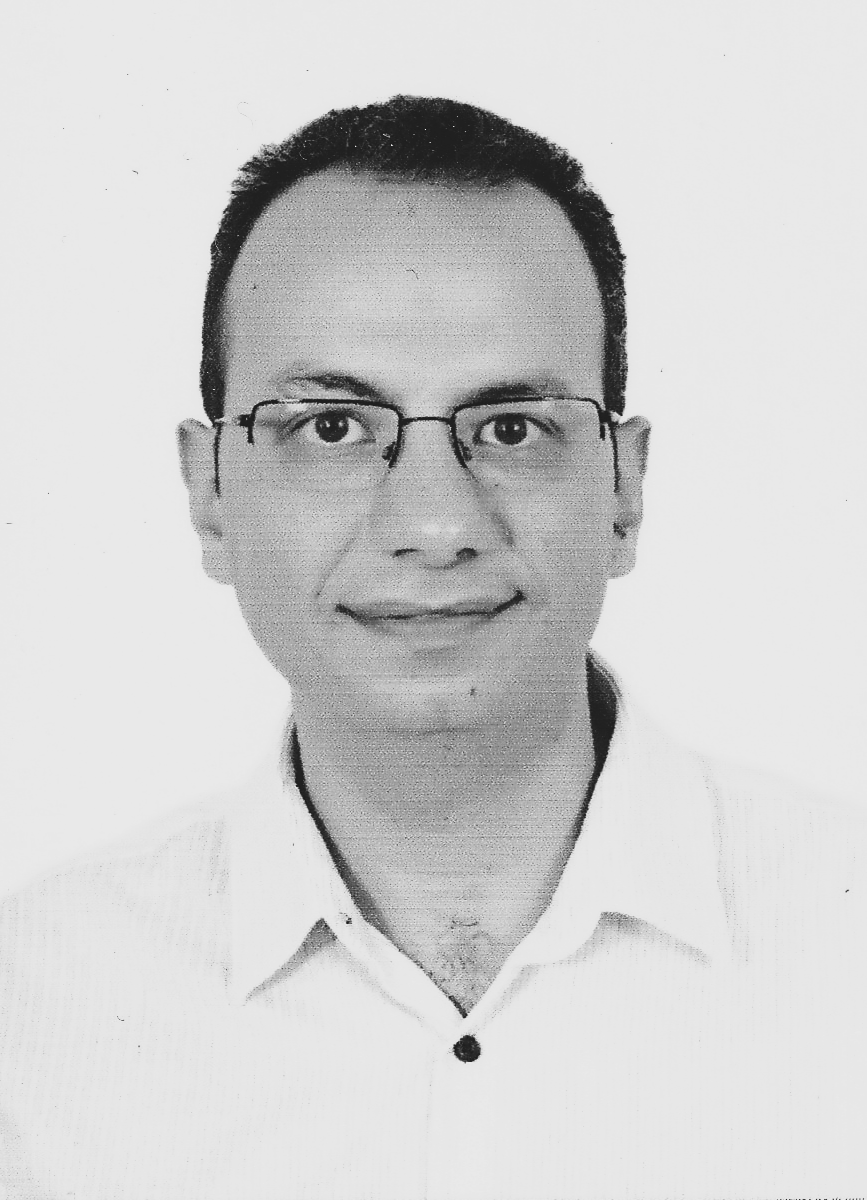
\includegraphics[width=1in,height=1.25in,clip,keepaspectratio]{Ahmed_gray.png}
\end{wrapfigure}
\noindent\textbf{Ahmed H. Abdel-Gawad} is an Associate Professor with the Computer Engineering Department, Faculty of Engineering, Cairo University, Giza, Egypt. His research spans machine learning, computer architecture and high performance computing. He supervised the work reported in this paper and contributed methodological guidance and critical revision of the manuscript.


\end{document}
